\documentclass[twocolumn]{el-author}

\usepackage{multirow}
\usepackage{pifont}
\usepackage{graphicx}
%\usepackage{subfigure}
\usepackage{IEEEtrantools}
\usepackage{subcaption}
\usepackage{caption}
\DeclareMathOperator\erf{erf}
\makeatletter
\DeclareRobustCommand\onedot{\futurelet\@let@token\@onedot}
\def\@onedot{\ifx\@let@token.\else.\null\fi\xspace}

\def\eg{\emph{e.g}\onedot} \def\Eg{\emph{E.g}\onedot}
\def\ie{\emph{i.e}\onedot} \def\Ie{\emph{I.e}\onedot}
\def\cf{\emph{c.f}\onedot} \def\Cf{\emph{C.f}\onedot}
\def\etc{\emph{etc}\onedot} \def\vs{\emph{vs}\onedot}
\def\wrt{w.r.t\onedot} \def\dof{d.o.f\onedot}
\def\etal{\emph{et al}\onedot}
\makeatother

\newcommand{\hH}{\hat{H}}
\newcommand{\D}{^\dagger}
\newcommand{\ua}{\uparrow}
\newcommand{\nc}{\newcommand}
\nc{\da}{\downarrow} \nc{\hc}{\hat{c}} \nc{\hS}{\hat{S}}
\nc{\bra}{\langle} \nc{\ket}{\rangle} \nc{\eq}{equation (\ref}
\nc{\h}{\hat} \nc{\hT}{\h{T}}\nc{\be}{\begin{eqnarray}}
\nc{\ee}{\end{eqnarray}}\nc{\rd}{\textrm{d}}\nc{\e}{eqnarray}\nc{\hR}{\hat{R}}\nc{\Tr}{\mathrm{Tr}}
\nc{\tS}{\tilde{S}}\nc{\tr}{\mathrm{tr}}\nc{\8}{\infty}\nc{\lgs}{\bra\ua,\phi|}\nc{\rgs}{|\ua,\phi\ket}
\nc{\hU}{\hat{U}}\nc{\lfs}{\bra\phi|}\nc{\rfs}{|\phi\ket}\nc{\hZ}{\hat{Z}}\nc{\hd}{\hat{d}}\nc{\mD}{\mathcal{D}}
\nc{\bd}{\bar{d}}\nc{\bc}{\bar{c}}\nc{\mc}{\mathcal}\nc{\ea}{eqnarray}\nc{\mG}{\mathcal{G}}\nc{\bce}{\begin{center}}
\nc{\ece}{\end{center}}
%\date{12th December 2011}

\begin{document}

\graphicspath{{figure/}}

\title{Optimal Fitting Polynomial For Linear Time Bilateral Filter}

\author{Longquan Dai, Mengke Yuan, Xiaopeng Zhang}

\abstract{The bilateral filter (BF) has demonstrated great effectiveness for a variety of problems. However, its brute-force implementation is time-consuming. One way of accelerating  BF is to approximate the nonlinear range kernel of BF by a set of linear time shiftable kernels. To reach this goal, we notice that only finite values of the kernel of BF are used to perform smoothing due to the quantization of digital images. Thus, it does not change the filtering results by substituting the range kernel with the function having the same values at finite discrete points. We also learn that the lagrange interpolation polynomial can exactly pass through predefined points and therefore employ it to replace the original kernels for accurate accelerating BF. In addition, for speeding up BF at the cost of small approximation error, two approximation methods are proposed to obtain the optimal fitting polynomial. The performance of our method is validated in extensive experiments. }

\maketitle

\section{Introduction}

The bilateral filter (BF)~\cite{Tomasi_ICCV_1998} is a valuable tool for many computer vision and graphics applications and its output at the pixel location $\bm{x} = (x, y)$ is given by
%
\begin{equation}
\hat{I}_{\bm{x}} = \frac{\sum_{\bm{y} \in \mathcal{N}^r_{\bm{x}}} K_s(\| \bm{y} - \bm{x} \|) K_r( I_{\bm{y}} - I_{\bm{x}} ) I_{\bm{y}}}{\sum_{\bm{y} \in \mathcal{N}^r_{\bm{x}}} K_s(\| \bm{y} - \bm{x} \|) K_r( I_{\bm{y}} - I_{\bm{x}} )}
\label{eq:BF}
\end{equation}
%
where $K_s(\cdot)$ is the spatial domain kernel, $K_r(\cdot)$ is the range kernel and $\mathcal{N}^r_{\bm{x}}$ is the square window centered at $\bm{x}$ with radius $r$. For BF, the kernels $K_s(\cdot)$ and $K_r(\cdot)$ determine how the spatial and intensity differences are treated. The most commonly used kernel in literature is the Gaussian kernel $G_{\sigma}(z) = \exp(-\frac{z^2}{2\sigma^2})$. Other unusual kernels are reported in~\cite{Durand_2002_TOG}. Due to the signal-dependant range kernel $K_r( I_{\bm{y}} - I_{\bm{x}} )$, BF becomes an edge-aware filter. On the flip side of the power, the complexity of the brute-force implementation is $O(|\mathcal{N}^r||I|)$ that is too intensive for time-critical applications, where $|I|$ is the number of pixels in the entire image and $|\mathcal{N}^r|$ is the number of pixels in the window $\mathcal{N}^r_{\bm{x}}$ centered at $\bm{x}$. The inefficiency stems from that the signal-dependant range kernel $K_r( I_{\bm{y}} - I_{\bm{x}} )$ introduces nonlinearity to BF and therefore rules out lots of fast calculating techniques. One solution is to approximate the nonlinear range kernel by a set of linear time shiftable kernels~\cite{Chaudhury_SPL_2011}, where the linear time means the computational complexity is $O(|{I}|)$ which is independent of the window radius $r$.
In literature, the existing accelerating methods of BF roughly fail into following two categories:

\begin{itemize}
\item \emph{\textbf{Series Expansion Based BF}}: This kind of BFs employ the Taylor series or linear time shiftable kernels~\cite{Chaudhury_SPL_2011} to represent the Gaussian range kernel. Chaudhury \etal~\cite{Chaudhury_TIP_2011} reduce the Gaussian kernel to the raised cosine range kernel. Dai~\etal~\cite{Dai_ET_2014} propose Hermite polynomials to decompose the Gaussian kernel. Our method also belongs to this kind of methods.
  \item \emph{\textbf{Histogram Based BF}} Porikli~\cite{Porikli_2008_CVPR} found that BF can be computed in linear time by the fast integral histogram~\cite{Porikli_CVPR_2005} if $K_s(\| \bm{y} - \bm{x} \|)$ is the box spatial kernel $B_{\mathcal{N}^{r}_{\bm{x}}}(\| \bm{y} - \bm{x} \|)$. Zhang \etal~\cite{Zhang_2012_TIP} use the de Moivre-Laplace theorem to decompose the Gaussian kernel into $M_s$ box functions.  Gunturk~\cite{Gunturk_TIP_2011} employs the least squares optimization to find the optimal coefficients $\beta^s_i$ that minimize the approximation error $(K_s(\| \bm{y} - \bm{x} \|) - \sum_{i = 1}^{M_s} \beta^s_i B_{\mathcal{N}^{r_i}_{\bm{x}}}(\| \bm{y} - \bm{x} \|))^2$. Pan~\etal~\cite{Pan_MPE_2014} formulate their objective function from the sparsity perspective to solve the optimal coefficients $\beta^s_i$.
\end{itemize}
%


\section{The Optimal Fitting Polynomial}

Since the intensity values of digital images are quantized to $N_r$ discrete values $r_j, 1 \leq j \leq N_r$, only finite discrete points $K_r(r_j)$ of BF's range kernel are used to compute the filtering results. We employ the least squares fitting algorithm to find the optimal fitting polynomial that approximates to the range kernel $K_r(\cdot)$ with the smallest approximation error at the discrete points $(r_j, K_r(r_j))$ and replace the range kernel $K_r(\cdot)$ in Eq.~\eqref{eq:BF} by the optimal polynomial. In this way,  the nonlinear convolution of $K_r(\cdot)$ can be decomposed into a set of box filters. More importantly, we can compute the box filter in linear time by the fast histogram technique~\cite{Porikli_CVPR_2005}.

In order to obtain a versatile fitting polynomial $P_r(\cdot)$, it is reasonable to expect that the optimal $P_r(z) = \sum_{i=0}^{M_r} \beta^r_i z^i $ can exactly pass through some predefined points in the set $\{(r_j, K_r(r_j))\}$ while minimizing the approximation error for the remaining points. Hence, we divide $\{(r_j, K_r(r_j))\}$ into two subsets, where the first $L$ points denote the points being used to compute the approximation error and the last $N_r-L$ points represent the predefined constrain points. Considering the two subsets, we employ the constrained quadratic optimization~\eqref{eq:obj_polynomial_constrain} to compute the  coefficients $\beta^r_i$ of the optimal fitting polynomial $P_r(\cdot)$.
%
\begin{equation}
\begin{split}
& \min_{\beta^r_i} \sum \nolimits_{j = 1}^{L} (K_{r}(r_j) - \sum \nolimits_{i=0}^{M_r} \beta^r_i (r_j)^i )^2 \\
& s.t. \quad
\begin{split}
& \sum \nolimits_{i=0}^{M_r} \beta^r_i (r_j)^i \ge 0, \quad 1 \leq  j \leq L \\
& \sum \nolimits_{i=0}^{M_r} \beta^r_i (r_j)^i = K_r(r_j), \quad L+1 \leq  j \leq N_r \\
\end{split}
\end{split}
\label{eq:obj_polynomial_constrain}
\end{equation}
%
The constrains $\sum \nolimits_{i=0}^{M_r} \beta^r_i (r_j)^i \ge 0$ are added to prevent negative fitting curve complained by Chaudhury~\cite{Chaudhury_TIP_2011}. Moreover, the optimization can be efficiently solved by the matlab function `lsqlin'.

\textbf{Case 1: $\bm{L =0}$.} The optimal polynomial  $P_r(\cdot)$ passes through all $N_r$ points in the set $\{(r_j, K_r(r_j))\}$ if the degree $M_r$ of the polynomial $P_r(\cdot)$ is no less than $N_r - 1$. Actually, employing the lagrange interpolation polynomial which is capable of exactly passing through all $N_r$ points in the set $\{(r_j, K_r(r_j))\}$, we can directly write down the closed form solution of the optimization~\eqref{eq:obj_polynomial_constrain} as
%
\begin{equation}
P_r(z) = \sum \nolimits^{N_r}_{i=1} K_r(r_i) \prod \nolimits_{j=1, j \neq i}^{N_r} \frac{z - r_j}{r_i - r_j}
\label{eq:Pr_lagrange}
\end{equation}
%
Although substituting the lagrange interpolation polynomial $P_r(\cdot)$ with $K_r(\cdot)$ does not change the filtering result, adopting it to speed up BF is not very efficient because the high degree polynomial increases the computation complexity. For instance, $r_j \in \{-255, \ldots,255\}$ for 8-bits image. In this situation, the degree of $P_r(\cdot)$ is up to $510$ which implies $510+$ times linear filtering for accelerating BF. One possible solution is to relax the exact equality constrains. %In other words, we find a fitting polynomial with a low degree to approximate all points in $\{(r_j, K_r(r_j))\}$. This corresponds to the case $ L = N_r$.

\textbf{Case 2: $ L = N_r$.} The optimal polynomial does not prefer any special points, and the constrained optimization~\eqref{eq:obj_polynomial_constrain} is free to decide the optimal polynomial $P_r(\cdot)$ with arbitrary degree. Although the produced $P_r(r_j)$ is no longer equal to $K_r(r_j)$, the approximation error is usually  very small. We can safely replace $K_r(r_j)$ by $P_r(r_j)$ without introducing significant numeric error. More importantly, the degree of $P_r(\cdot)$ will be very low  compared with the lagrange polynomial. However, when $ L = N_r$, Eq.~\eqref{eq:obj_polynomial_constrain} is not appropriate to compute the optimal fitting curve for nonsmoothing range kernel $K_r(\cdot)$.

 %In the nonsmoothing case, we usually hope the optimal polynomial $P_r(\cdot)$ exactly equals to $K_r(\cdot)$ at the nonsmoothing points and approaches to $K_r(\cdot)$ at the smoothing points because the maximal approximation error of the smoothing polynomial usually achieves at the nonsmoothing points. We do this by putting $0 < L < N_r$.

\textbf{Case 3: $0 < L < N_r$.} The optimal polynomial $P_r(\cdot)$ exactly passes through the last $N_r-L$ predefined points in the set $\{(r_j, K_r(r_j))\}$ with the smallest approximation error for the first $L$ points in the set $\{(r_j, K_r(r_j))\}$, if the degree $M_r \geq N_r-L-1$. Note that the optimal polynomial $P_r(\cdot)$ is a compromise for the first two cases. In the first case, $P_r(\cdot)$ produces accurate values at the cost of high degree (\ie high computational burden). Although the optimal $P_r(\cdot)$ in the second case achieves the lowest degree, its value is not accurate. The third case makes a compromise between the degree (efficiency) and the number of the accurate values (accuracy).

Frankly, all three cases have pros and cons. Users can choose different solutions according to different requirements. Here, we provide an unified framework that is able to trade off the efficiency and accuracy for different situations.

\section{Our Accelerating method}

We employ the optimal polynomial $P_r(z) = \sum_{i = 0}^{M_r}  \beta^r_i z^i$ with degree $M_r$ to approximate arbitrary range kernel $K_r(\cdot)$ as $P_r(z)$ is able to linearize the nonlinear convolution of $K_r(\cdot)$. Then, substituting the nonlinear convolution of $K_r(\cdot)$ with $P_r(z)$, we have
%
\begin{equation}
\hat{I}_{\bm{x}} = \frac{\sum_{i = 0}^{M_r} \sum_{j = 0}^{i} \varphi_{ij} (I_{\bm{x}}) \sum_{\bm{y} \in \mathcal{N}^{r}_{\bm{x}}} K_{s}(\|\bm{y}-\bm{x}\|)  F^{ij}_{\bm{y}} }{\sum_{i = 0}^{M_r} \sum_{j = 0}^{i} \varphi_{ij}(I_{\bm{x}}) \sum_{\bm{y} \in \mathcal{N}^{r}_{\bm{x}}} K_{s}(\|\bm{y}-\bm{x}\|) }
\label{eq:BF_approx_expansion_dai_aux}
\end{equation}
%
where $\varphi_{ij}(I_{\bm{x}}) = \beta^r_i {i \choose j} (-I_{\bm{x}})^{i-j} $, $\psi_{ij}(I_{\bm{y}}) = I^j_{\bm{y}} $ and $F^{ij}_{\bm{y}} =  \psi_{ij}(I_{\bm{y}})  I_{\bm{y}}$. Once again, the most time-consuming operation in Eq.~\eqref{eq:BF_approx_expansion_dai_aux} is the linear convolution of $K_{s}(\cdot)$ because $\sum_{i = 0}^{M_r} \sum_{j = 0}^{i}$ is pointwise sum operation.

In literature, the Fast Fourier transform is exploited to fast compute the linear convolution. We can also employ Pan's multiple boxes approximation strategy~\cite{Pan_MPE_2014} to compute the filtering results. According to Pan's method, we decompose the spatial kernel $K_s(\| \bm{y} - \bm{x} \|)$ into $M_s$ box functions $K_s(\| \bm{y} - \bm{x} \|) \approx \sum_{i = 1}^{M_s} \beta^s_i B_{\mathcal{N}^{r_i}_{\bm{x}}}(\| \bm{y} - \bm{x} \|)$, where $B_{\mathcal{N}^{r}_{\bm{x}}}(\| \bm{y} - \bm{x} \|) = 1$ when $\bm{y} \in \mathcal{N}^{r}_{\bm{x}}$, otherwise $B_{\mathcal{N}^{r}_{\bm{x}}}(\| \bm{y} - \bm{x} \|) = 0$. Then replacing the nonlinear convolution by $\sum_{i = 1}^{M_s} \beta^s_i B_{\mathcal{N}^{r_i}_{\bm{x}}}(\| \bm{y} - \bm{x} \|)$, we can obtain the fast equivalent filtering form~\eqref{eq:BF_approx_expansion_dai}.
%
\begin{equation}
\hat{I}_{\bm{x}} = \frac{\sum_{i = 0}^{M_r} \sum_{j = 0}^{i} \varphi_{ij} (I_{\bm{x}}) \sum_{k = 1}^{M_s} \beta^s_k  \mathcal{B}^{\mathcal{N}_{\bm{x}}}_{  F^{ij}  }   }{\sum_{i = 0}^{M_r} \sum_{j = 0}^{i} \varphi_{ij}(I_{\bm{x}}) \sum_{k = 1}^{M_s} \beta^s_k   \mathcal{B}^{\mathcal{N}_{\bm{x}}}_{ E } }
\label{eq:BF_approx_expansion_dai}
\end{equation}
%
The integral histogram technique can compute the box filtering results $\mathcal{B}^{\mathcal{N}_{\bm{x}}}_{  F^{ij} }$ and $\mathcal{B}^{\mathcal{N}_{\bm{x}}}_{ E }$ of $F^{ij}$ and the matrix $E$ of
ones. Moreover, the sum operations $\sum_{i = 0}^{M_r} \sum_{j = 0}^{i}, \sum_{k = 1}^{M_s} $ are pointwise. Hence the overall computational complexity of Eq.~\eqref{eq:BF_approx_expansion_dai} is $O(|I|)$.


\section{Kernel Approximation}


\begin{figure}[t]
\centering
\begin{subfigure}[b]{0.32\linewidth}
    \centering
    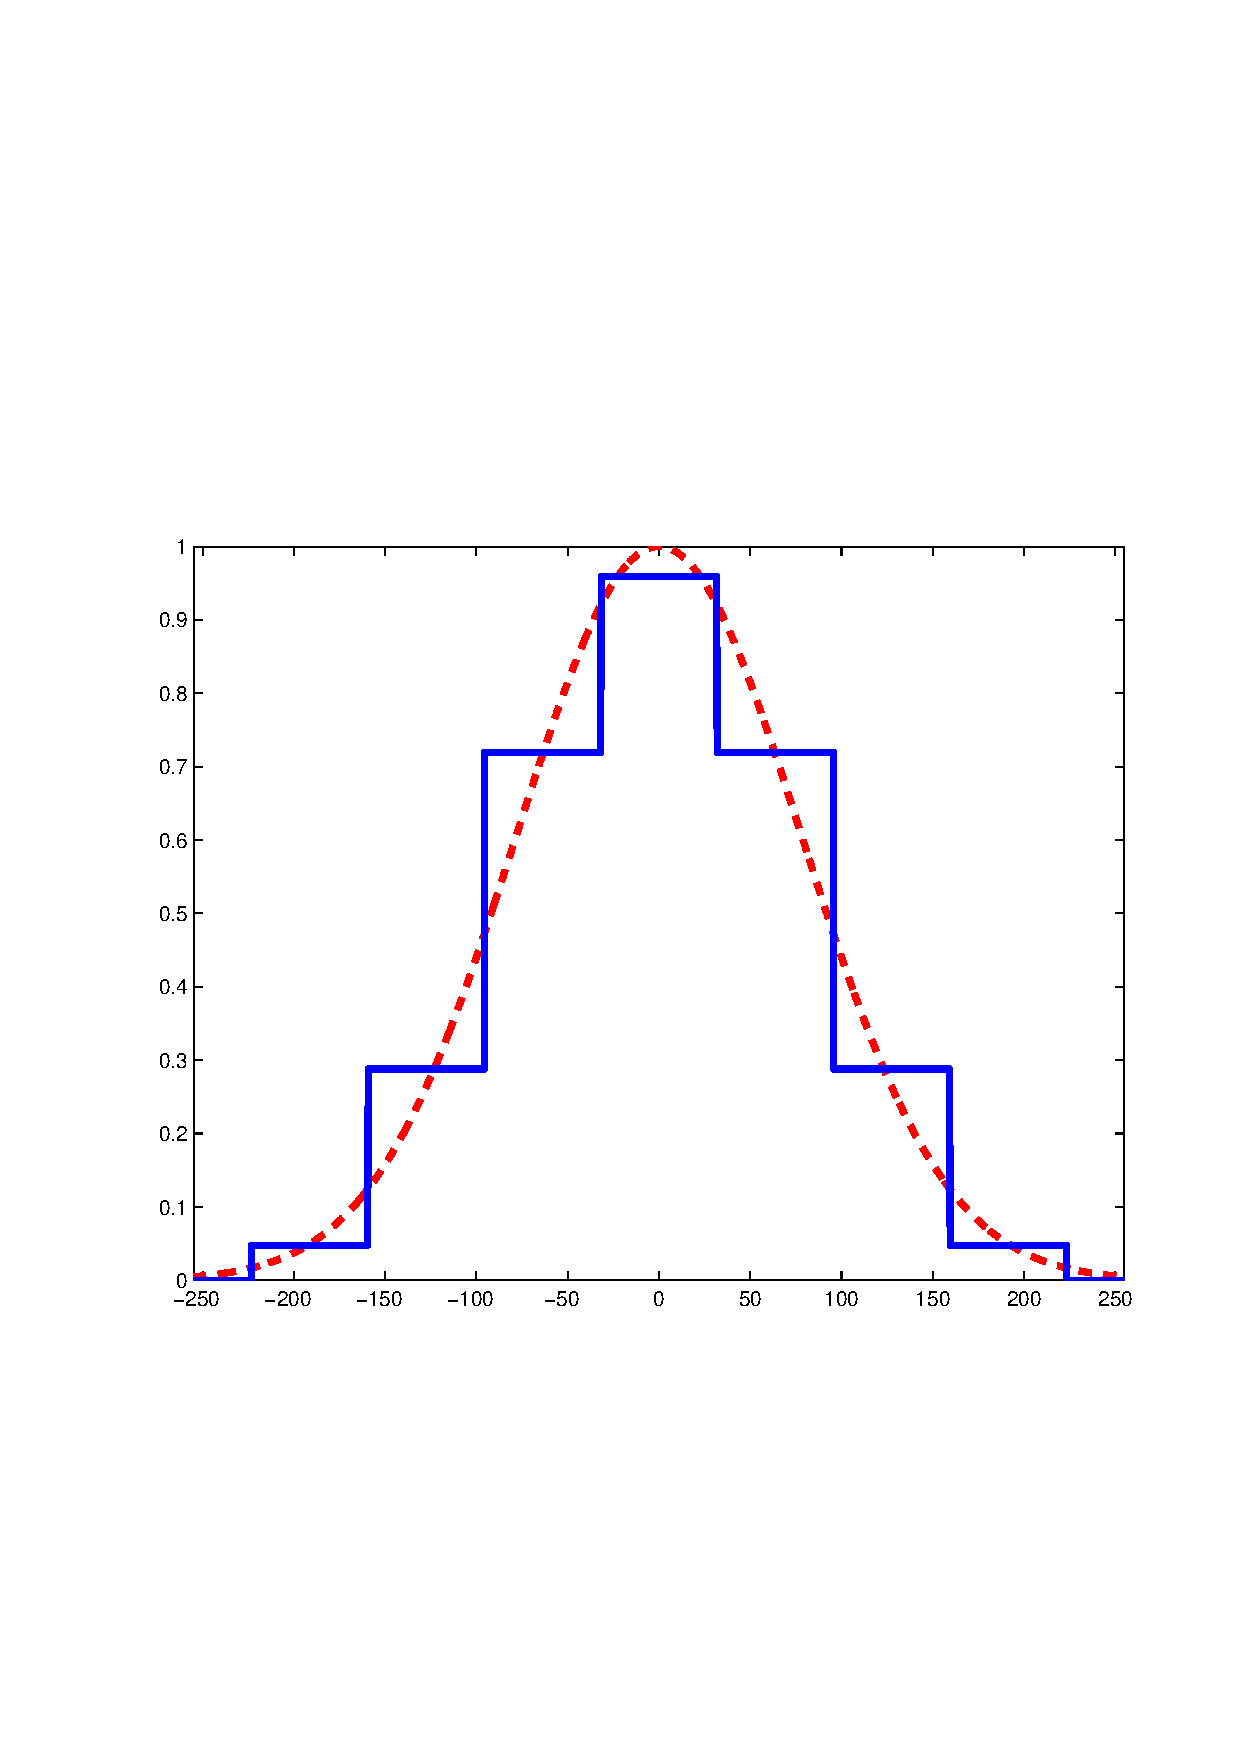
\includegraphics[width=\linewidth, height= 0.6\linewidth]{zhang1}
    %\captionsetup{skip=1pt}
    \caption{Zhang~\cite{Zhang_2012_TIP}}
    \label{fig:minimax_path:path}
\end{subfigure}
\hfill
\begin{subfigure}[b]{0.32\linewidth}
    \centering
    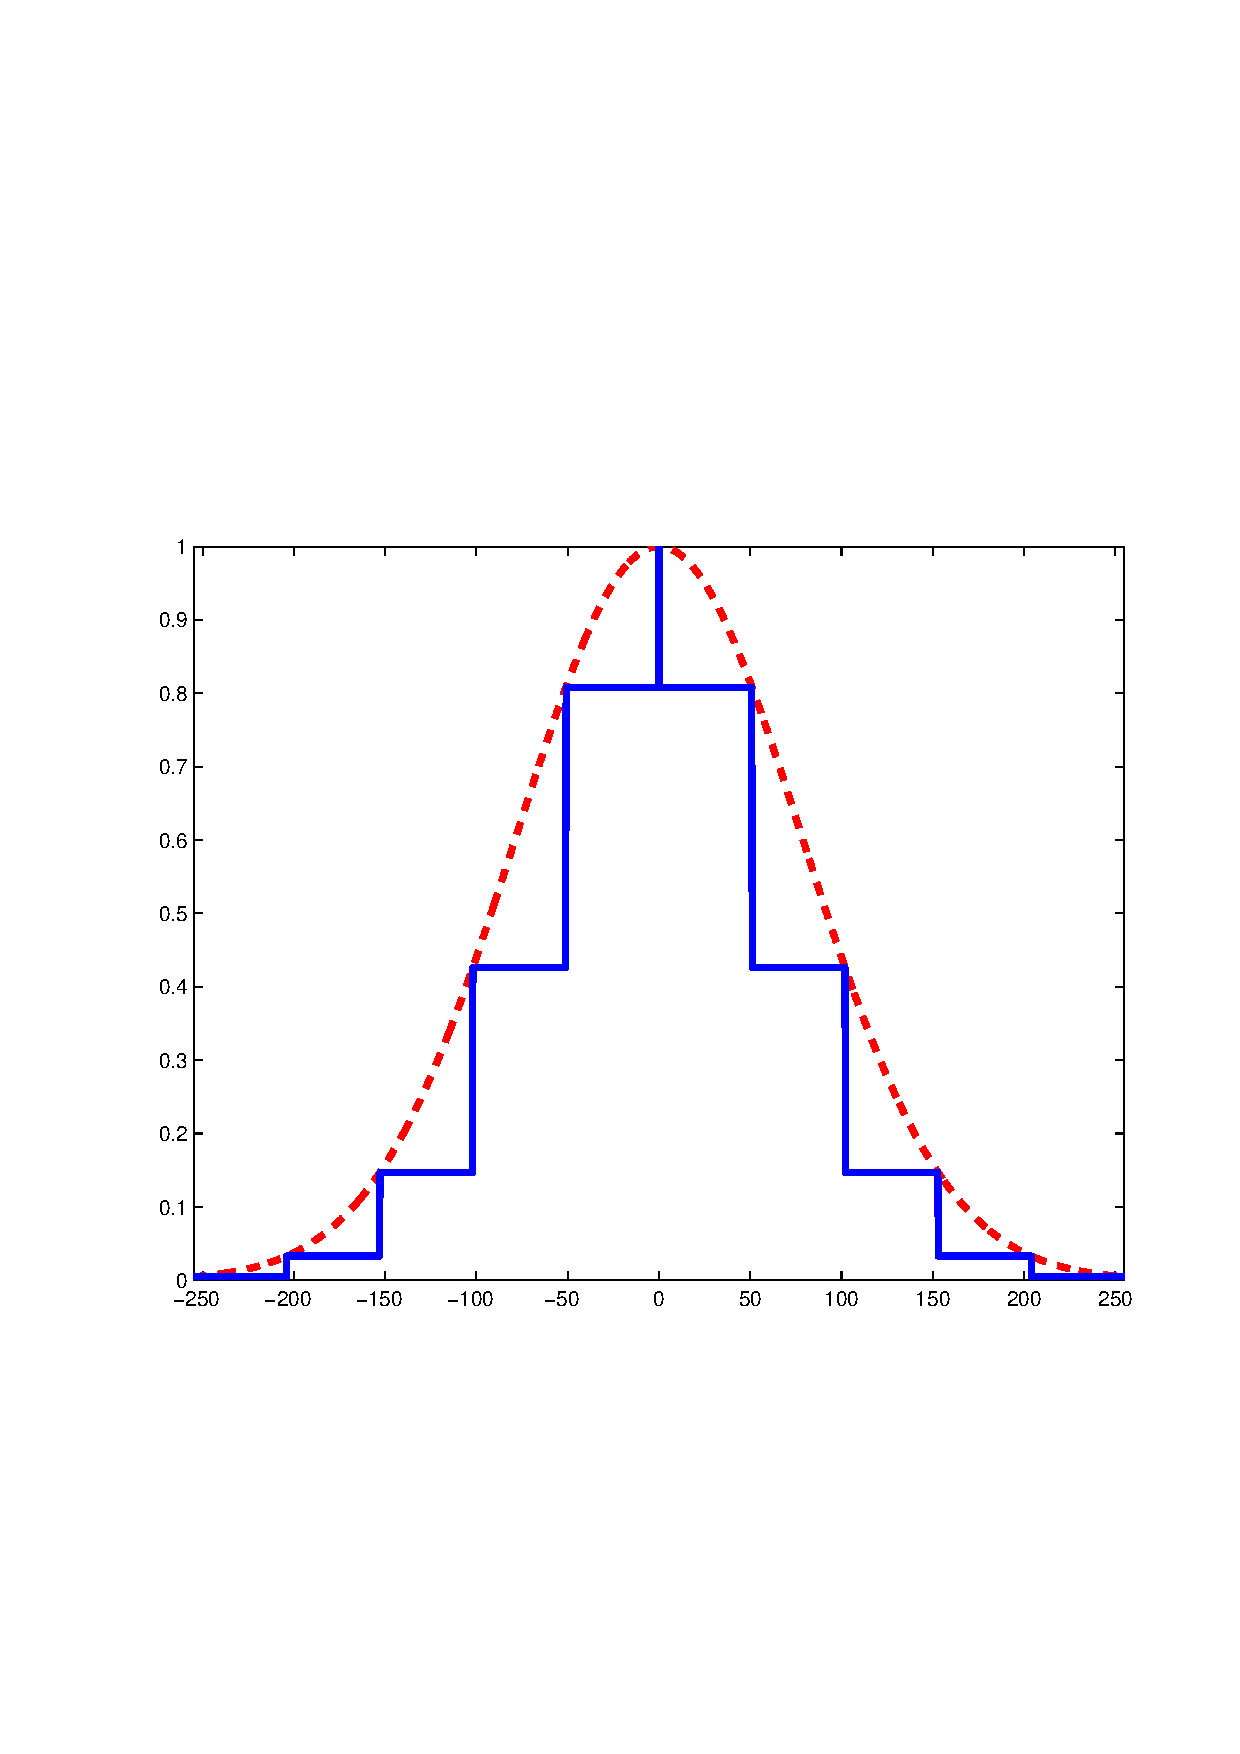
\includegraphics[width=\linewidth, height= 0.6\linewidth]{Gunturk1}
    %\captionsetup{skip=1pt}
    \caption{Gunturk~\cite{Gunturk_TIP_2011}}
    \label{fig:minimax_path:path}
\end{subfigure}
\hfill
\begin{subfigure}[b]{0.32\linewidth}
    \centering
    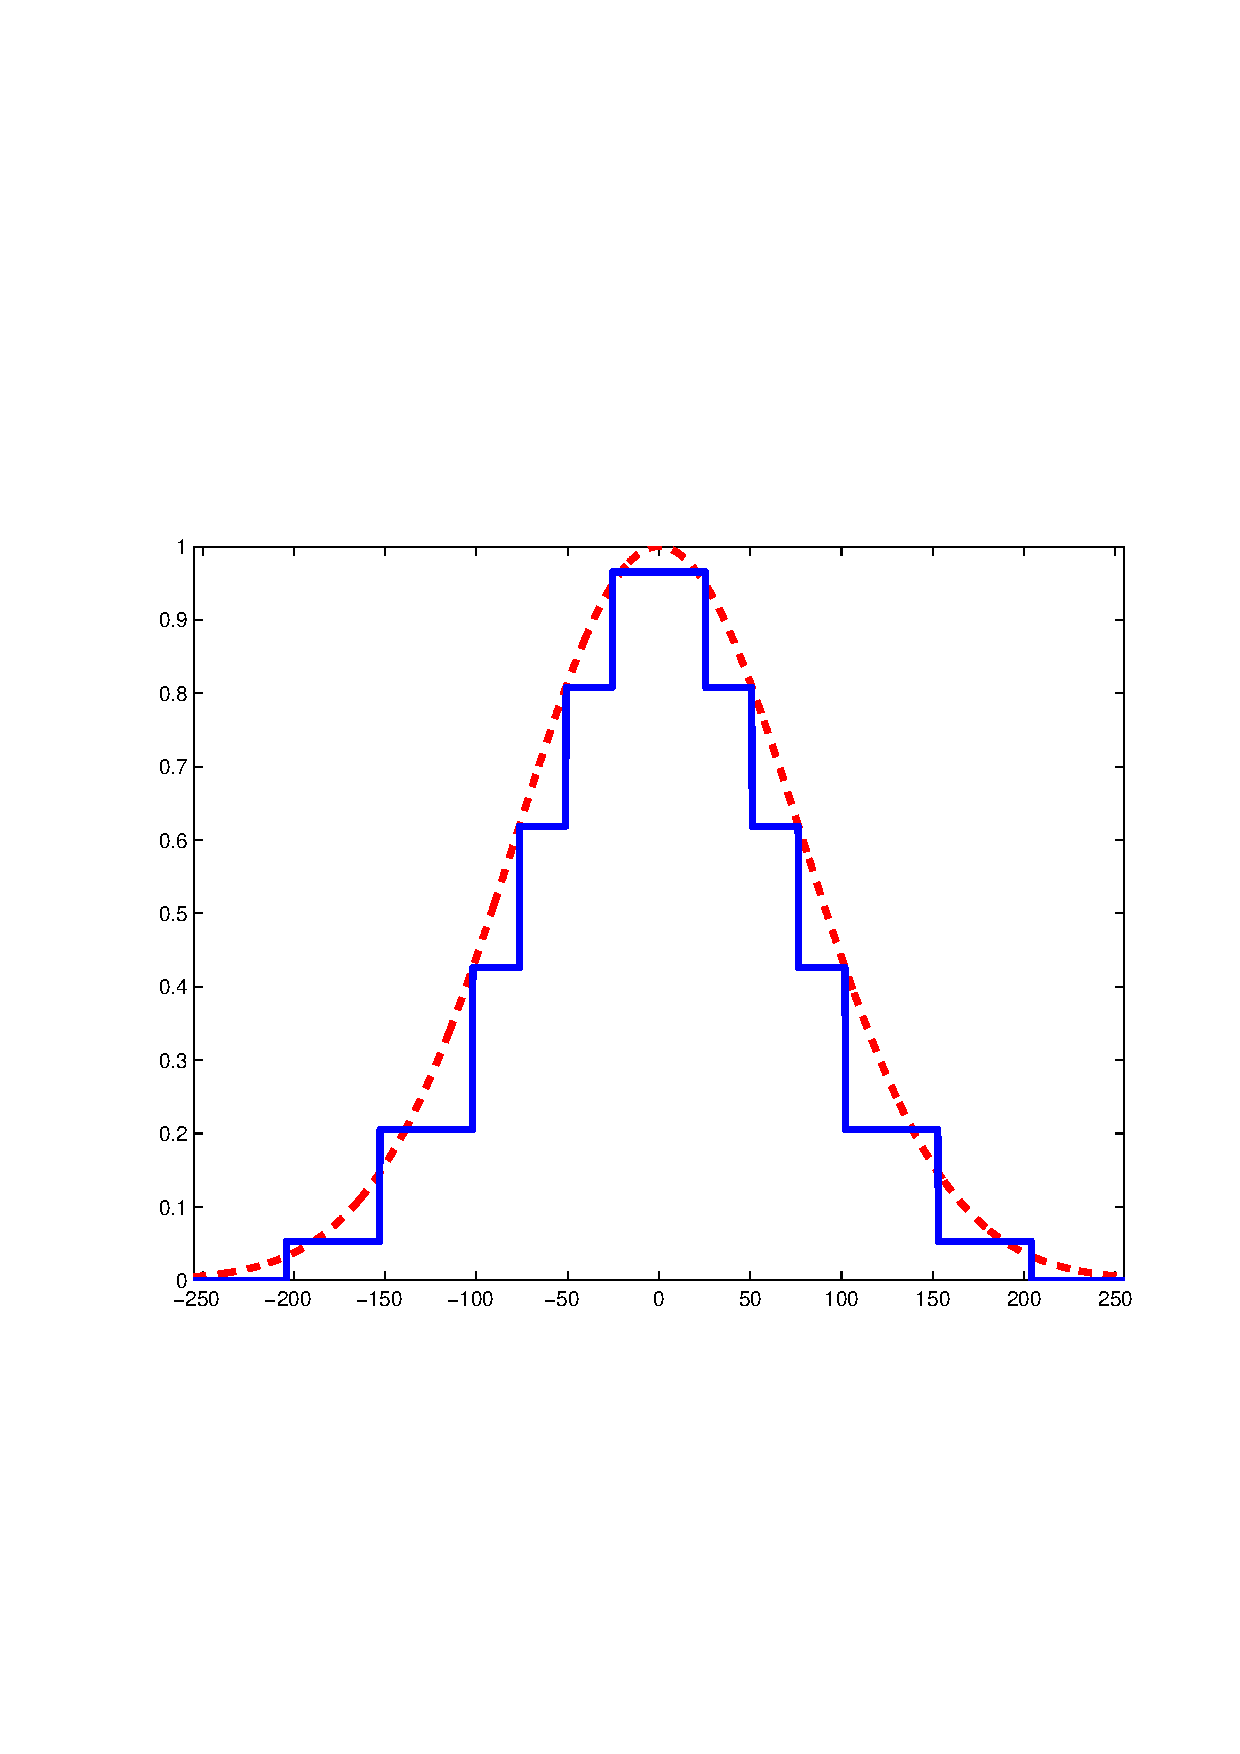
\includegraphics[width=\linewidth, height= 0.6\linewidth]{Pan1}
    %\captionsetup{skip=1pt}
    \caption{Pan~\cite{Pan_MPE_2014}}
    \label{fig:minimax_path:path}
\end{subfigure}

\begin{subfigure}[b]{0.32\linewidth}
    \centering
    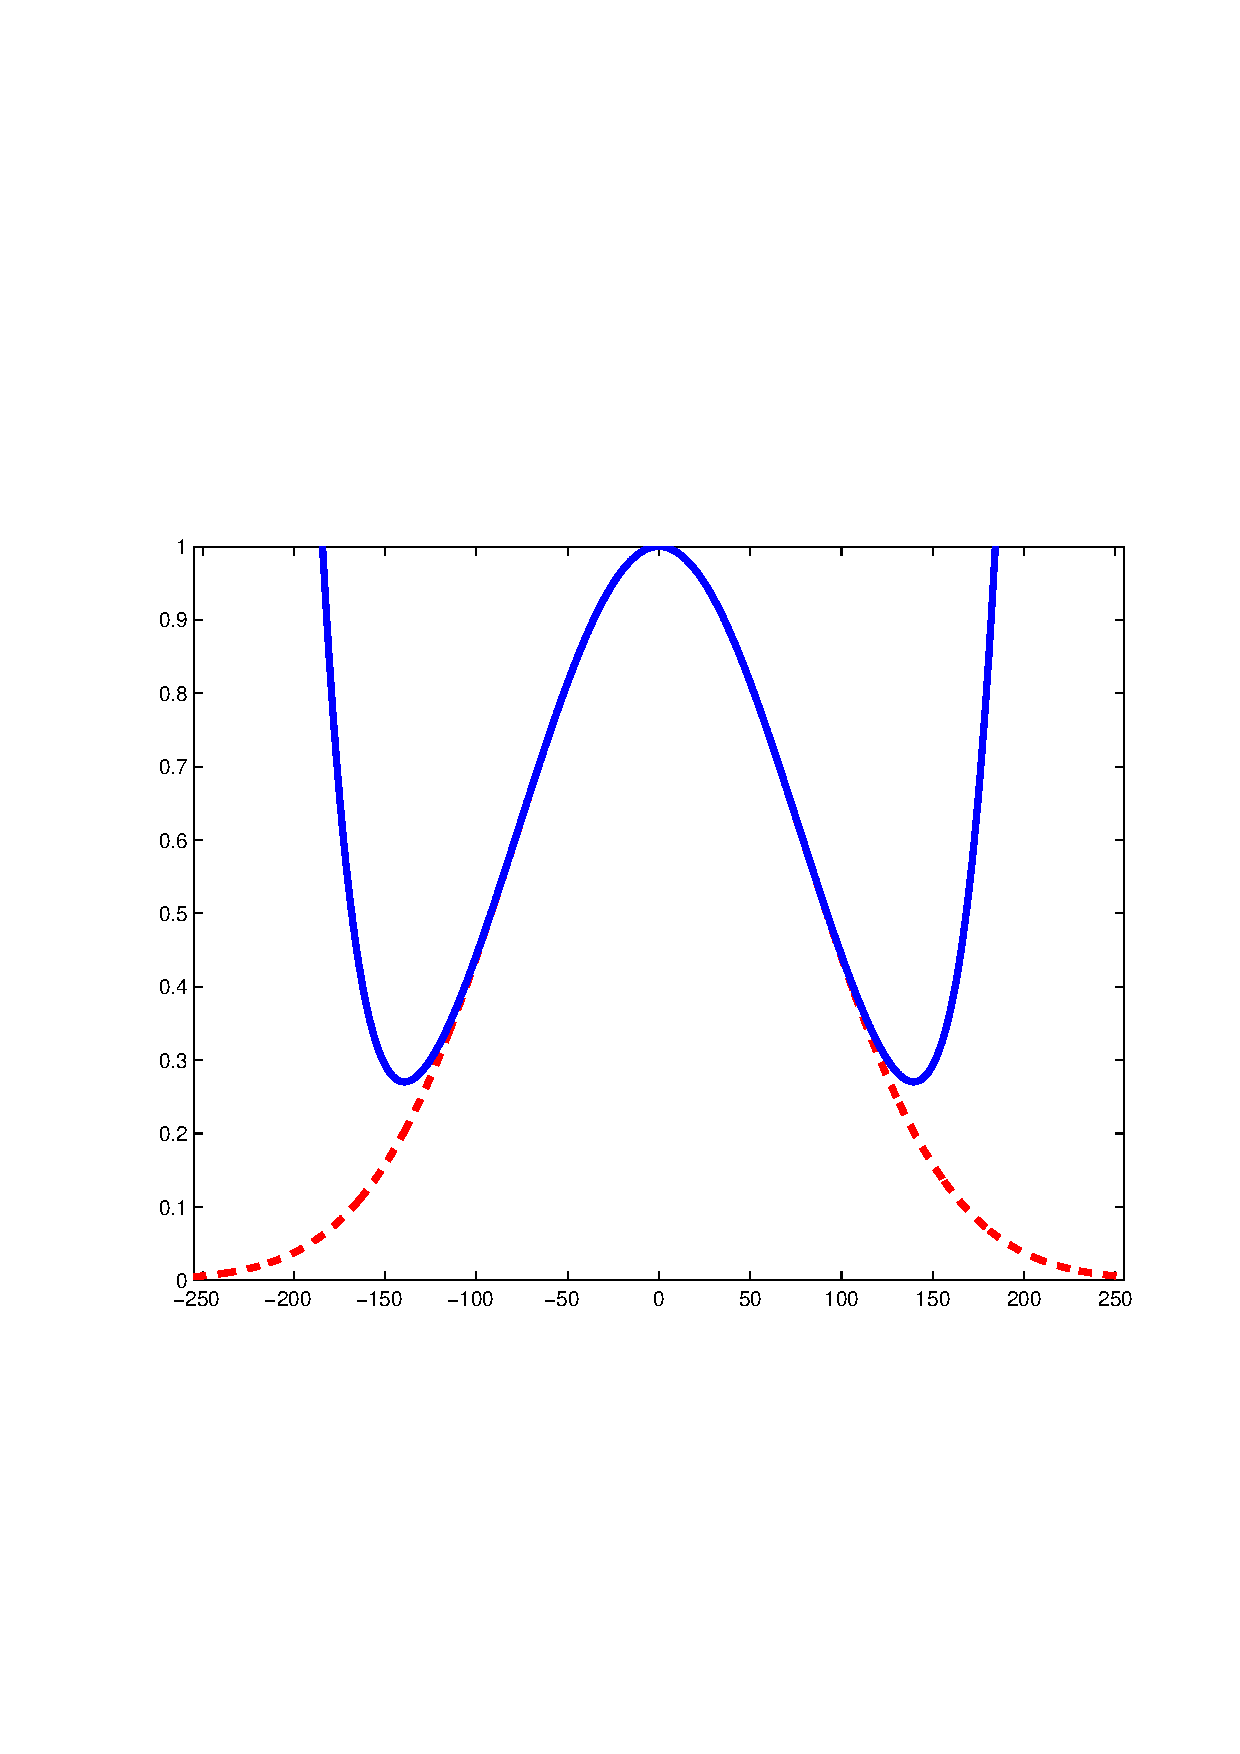
\includegraphics[width=\linewidth, height= 0.6\linewidth]{Porikli1}
    %\captionsetup{skip=1pt}
    \caption{Dai~\cite{Dai_ET_2014}}
    \label{fig:minimax_path:path}
\end{subfigure}
\hfill
\begin{subfigure}[b]{0.32\linewidth}
    \centering
    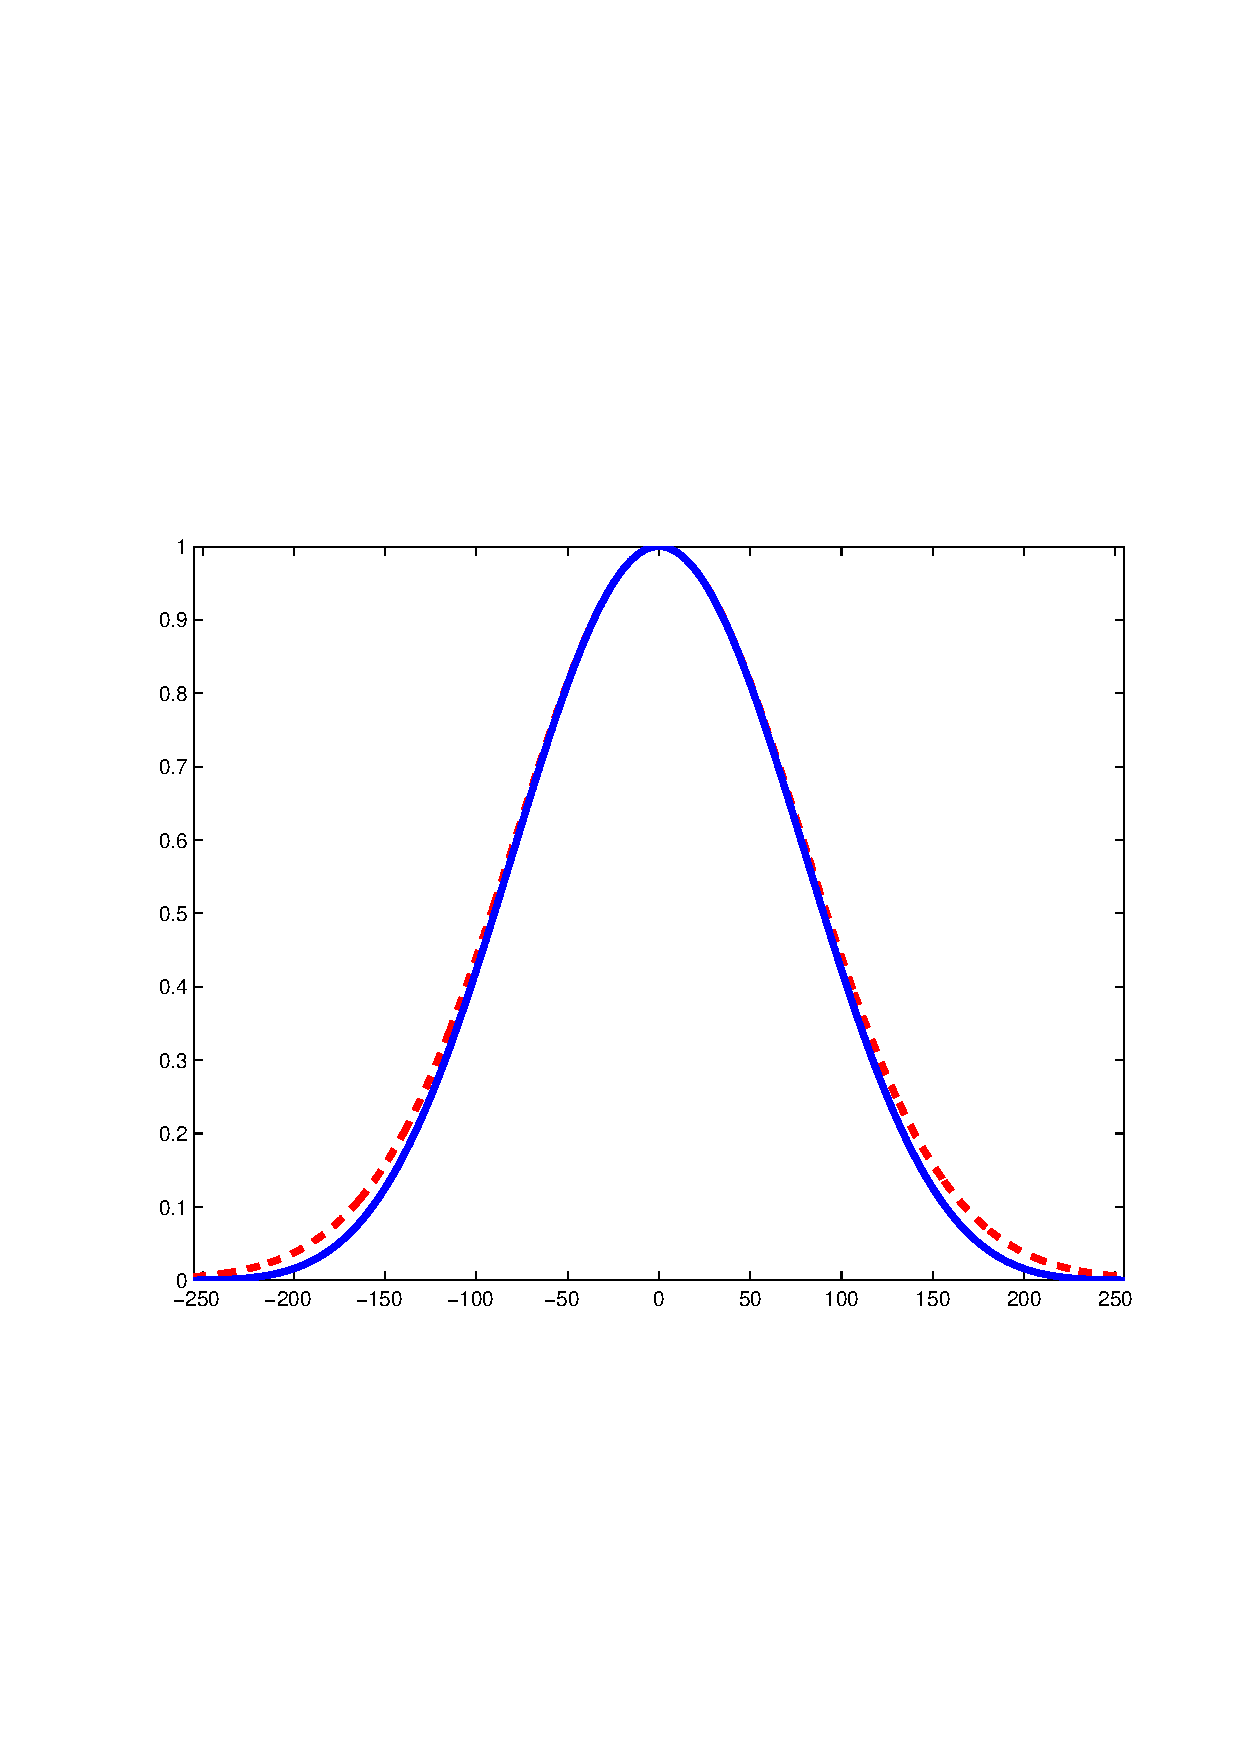
\includegraphics[width=\linewidth, height= 0.6\linewidth]{Chaudhury1}
    %\captionsetup{skip=1pt}
    \caption{Chaudhury~\cite{Chaudhury_TIP_2011}}
    \label{fig:minimax_path:path}
\end{subfigure}
\hfill
\begin{subfigure}[b]{0.32\linewidth}
    \centering
    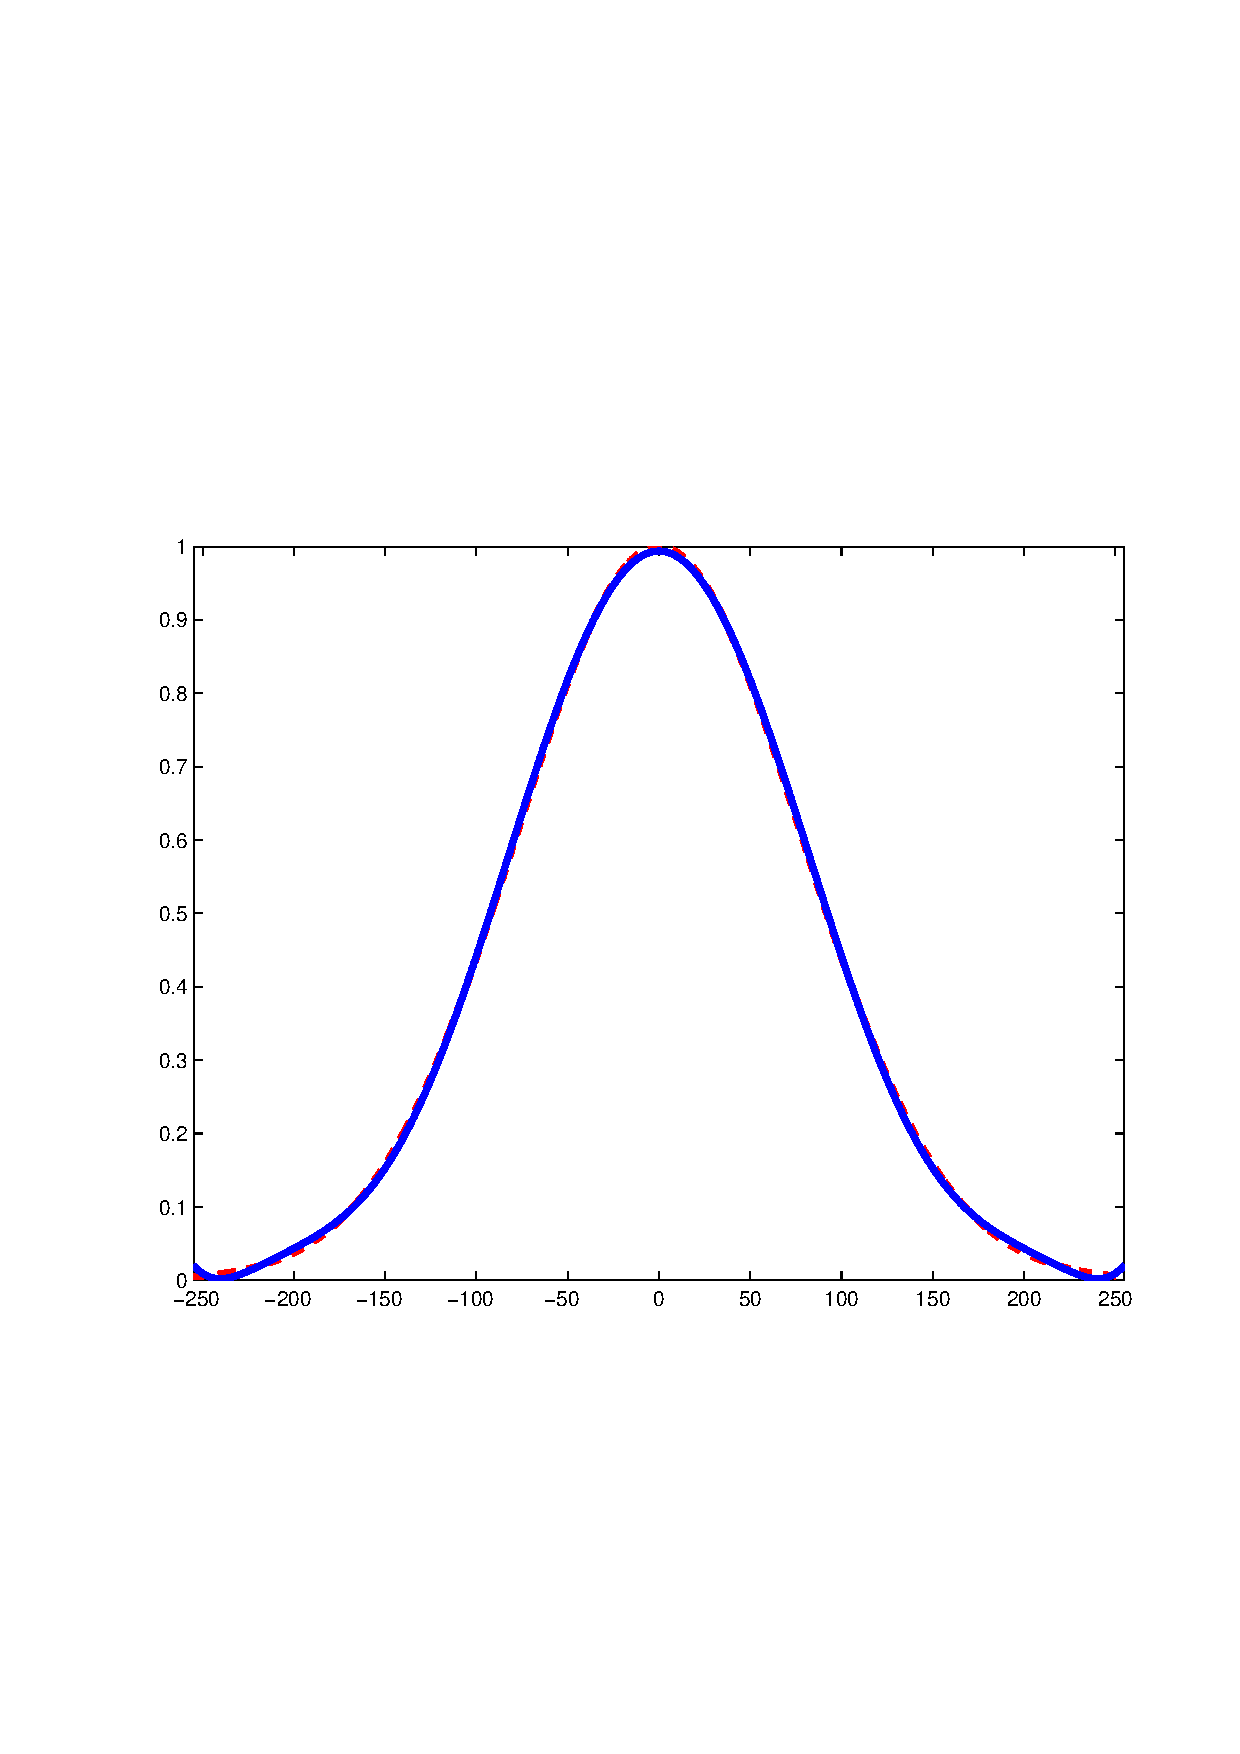
\includegraphics[width=\linewidth, height= 0.6\linewidth]{ours1}
    %\captionsetup{skip=1pt}
    \caption{Ours}
    \label{fig:minimax_path:path}
\end{subfigure}

\begin{subfigure}[b]{0.32\linewidth}
    \centering
    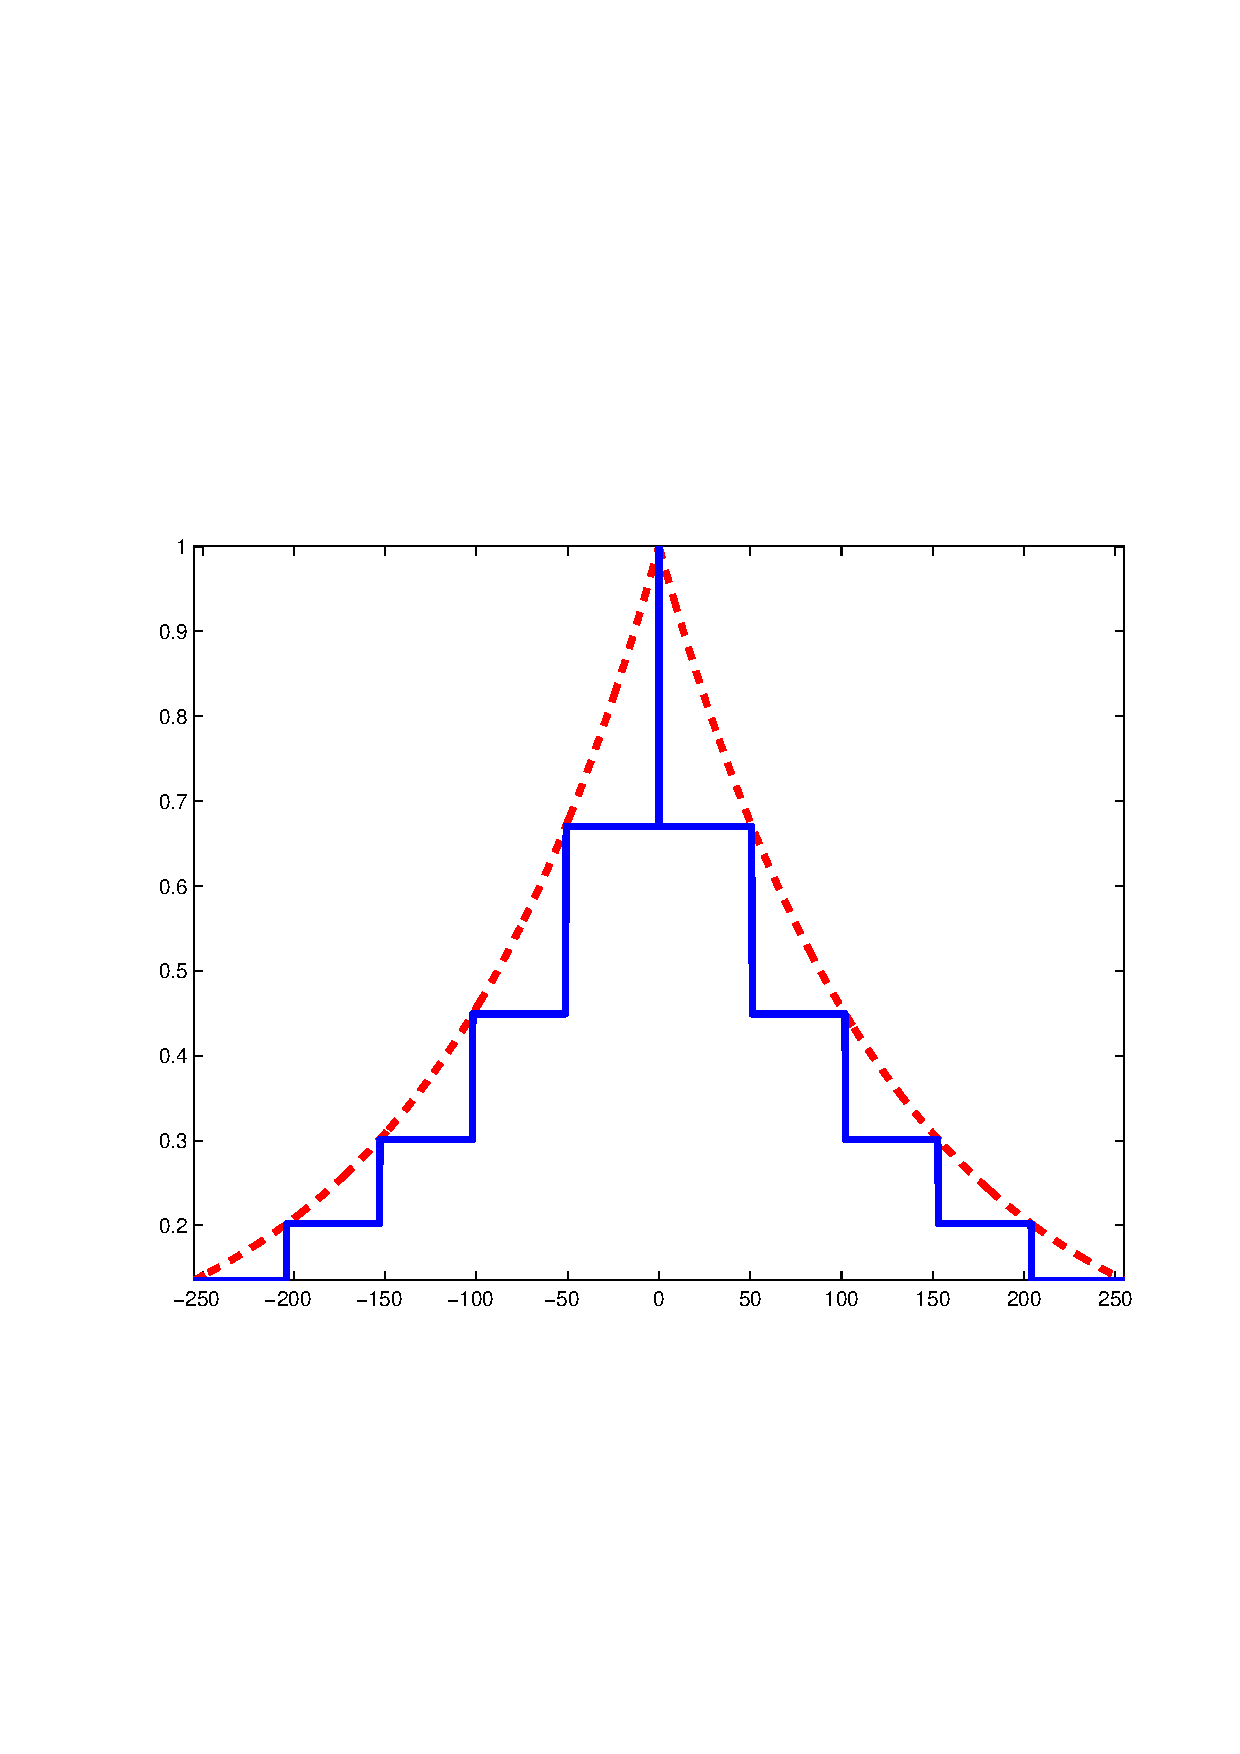
\includegraphics[width=\linewidth, height= 0.6\linewidth]{f2Gunturk1}
    %\captionsetup{skip=1pt}
    \caption{Gunturk~\cite{Gunturk_TIP_2011}}
    \label{fig:minimax_path:path}
\end{subfigure}
\hfill
\begin{subfigure}[b]{0.32\linewidth}
    \centering
    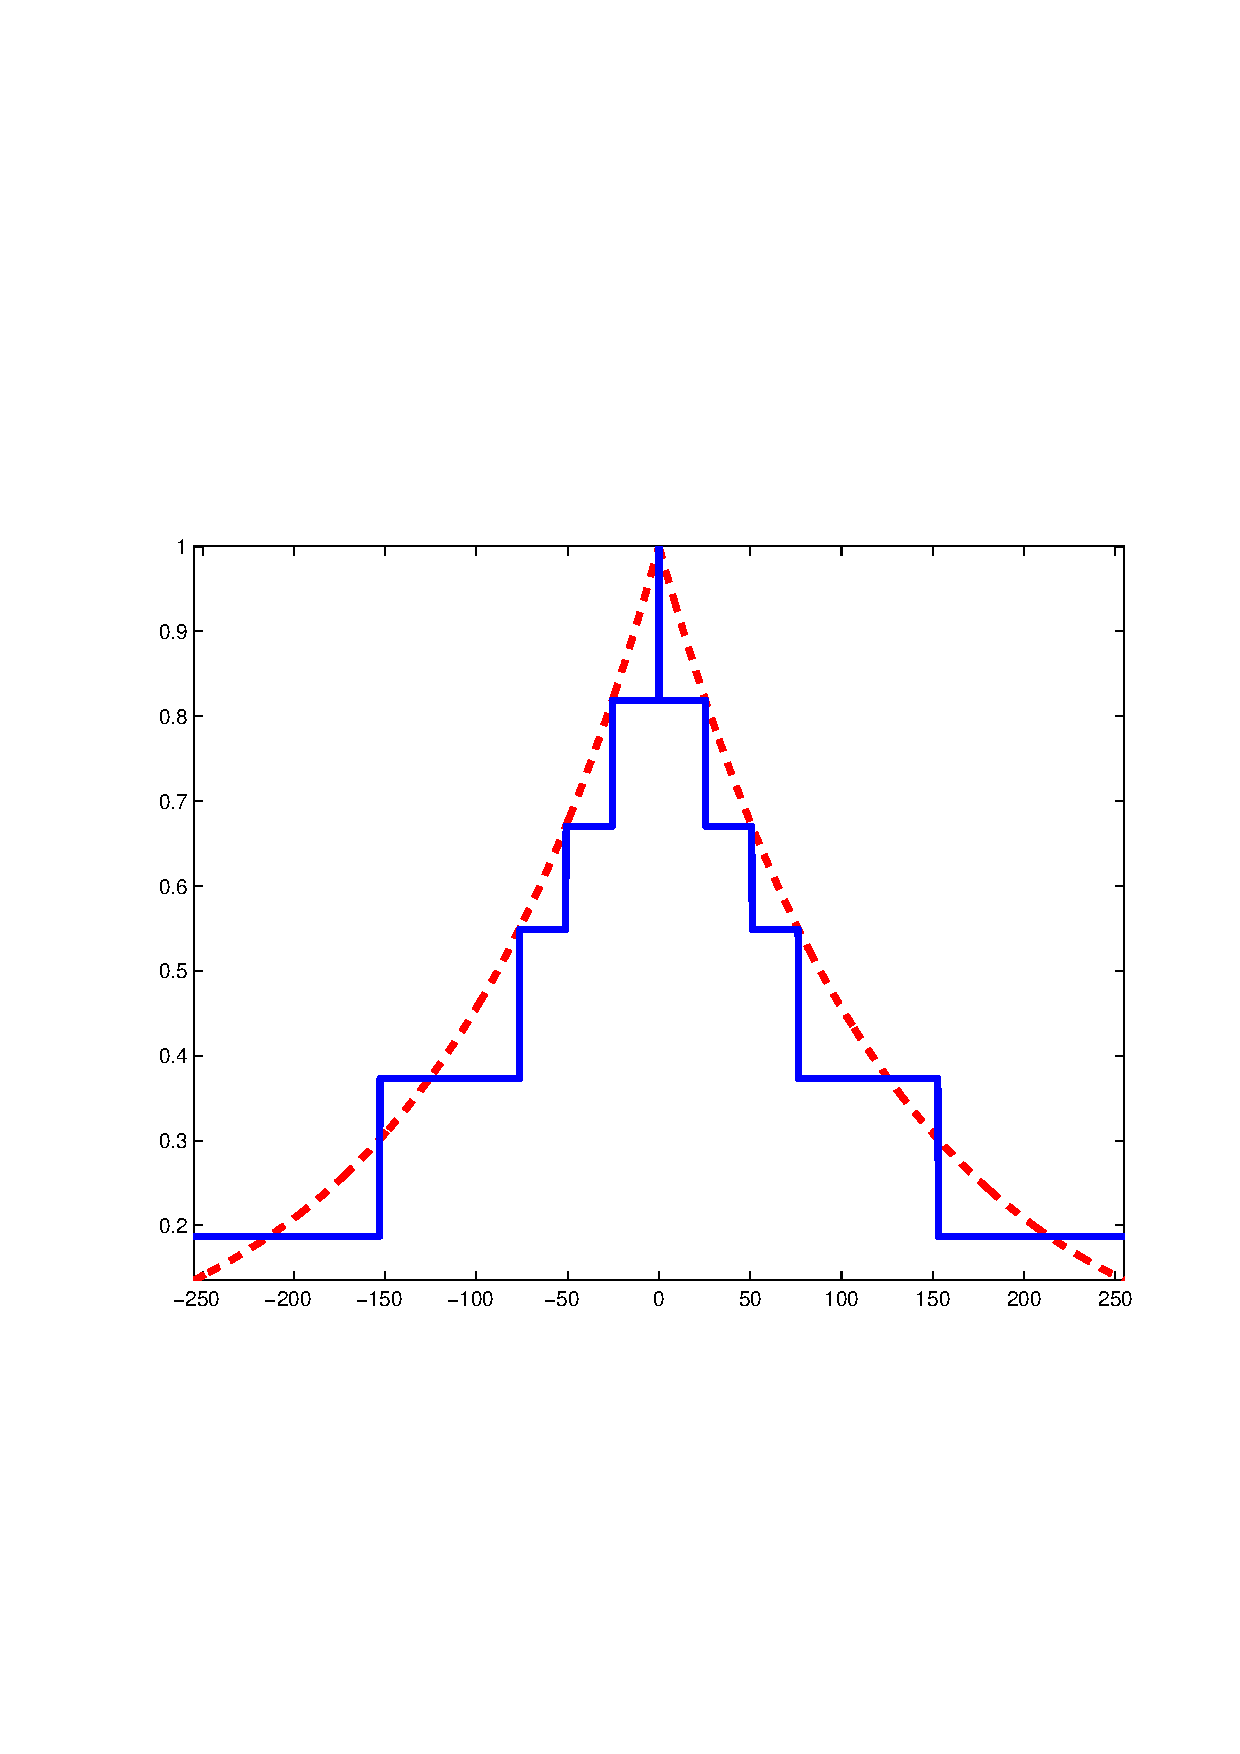
\includegraphics[width=\linewidth, height= 0.6\linewidth]{f2Pan1}
    %\captionsetup{skip=1pt}
    \caption{Pan~\cite{Pan_MPE_2014}}
    \label{fig:minimax_path:path}
\end{subfigure}
\hfill
\begin{subfigure}[b]{0.32\linewidth}
    \centering
    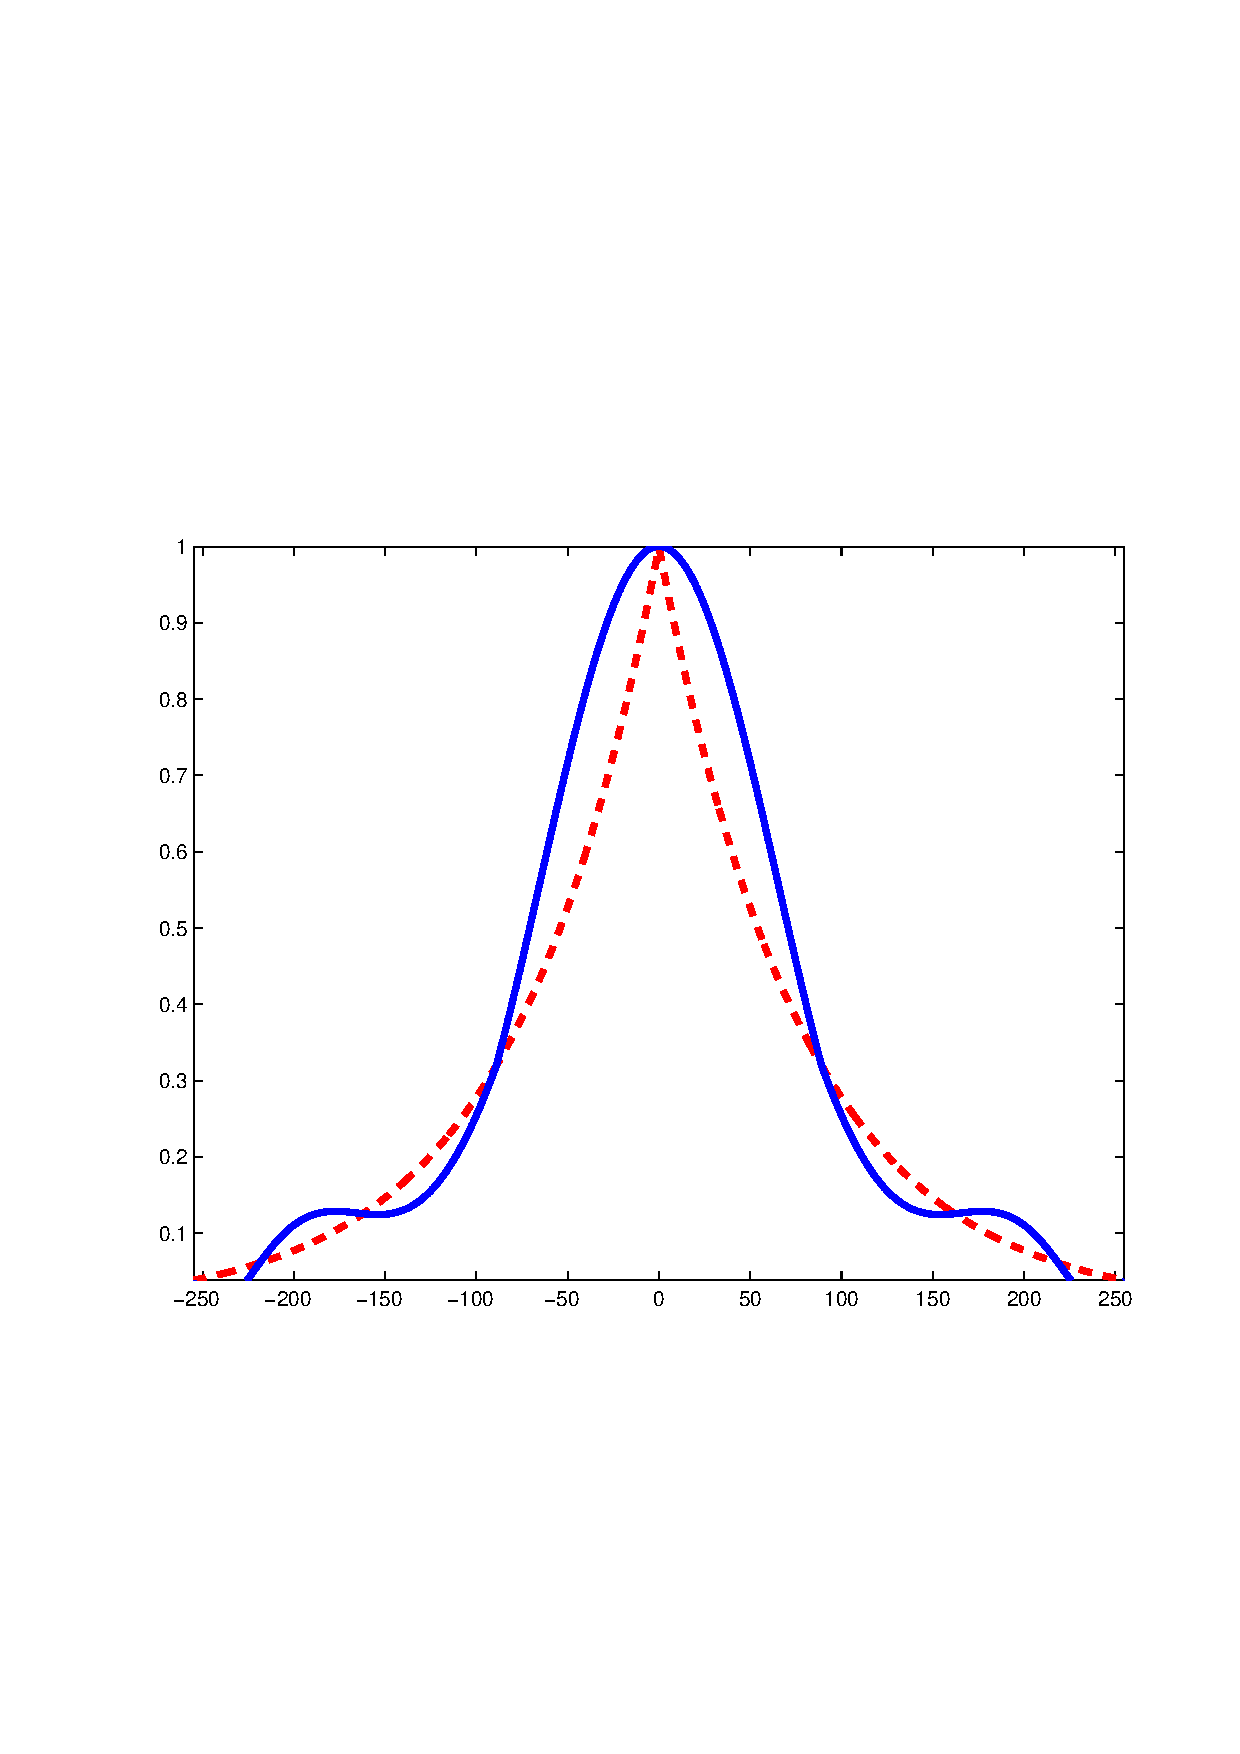
\includegraphics[width=\linewidth, height= 0.6\linewidth]{f2ours1}
    %\captionsetup{skip=1pt}
    \caption{Ours}
    \label{fig:minimax_path:path}
\end{subfigure}
\caption{The Gaussian kernel approximations (in the first and second rows) and the exponential decay kernel $\exp(-\frac{|x|}{\sigma})$  approximations (in the third row), where the variance $\sigma=80$.
}
\label{fig:gaussian}
\vspace{-0.1cm}
\end{figure}

BF accelerating methods usually decompose BF into a set of linear time filters for fast computation. They do this by substituting the original kernel in BF with its approximation. Thereby the accuracy of the approximation kernel determines the accuracy of final results. In literature, Zhang~\cite{Zhang_2012_TIP}, Gunturk~\cite{Gunturk_TIP_2011} and Pan~\cite{Pan_MPE_2014} all resort to a set of box functions to approximate the Gaussian kernel. The major difference is that the three methods take different techniques to determine the radiuses $r_i$ of box functions and the coefficients $\beta^s_i$. However, due to the nonsmooth property, the box functions can only obtain rough approximations for the Gaussian kernel as illustrated in Fig~\ref{fig:gaussian}. In contrast, Dai~\cite{Dai_ET_2014} and Chaudhury~\cite{Chaudhury_TIP_2011} take advantage of the Hermite polynomials and raised cosines, respectively, to approximate the Gaussian kernel. Nevertheless, the success of series expansion methods depends on the smoothness of the target kernel. For arbitrary nonsmooth kernels, there is no guarantee for the existence of series expansion. Even worse, the approximation for the Gaussian kernel with small variance is not satisfactory. The approximation errors of both two series expansion methods are significant using a low order expansion, when the variance of the Gaussian kernel is small. Moreover, the approximation using the box function is also not very well for the small variance. Since there are no special points on the curve of the smooth Gaussian kernel, we choose the second case in the The Optimal Fitting Polynomial section to compute the optimal polynomial of the Gaussian kernel and illustrate the optimal polynomial with degree $6$ for the $511$ discrete points $\{(r_i, G_{\sigma}(r_i))\}, r_i \in \{-255, \ldots, 255 \}$ in Fig.~\ref{fig:approximation_error}.


The exponential decay kernel $\exp(-\frac{|x|}{\sigma})$ is not differentiable at zero. The methods of Zhang~\cite{Zhang_2012_TIP}, Dai~\cite{Dai_ET_2014} and Chaudhury~\cite{Chaudhury_TIP_2011} can not deal with this situation. Although the box function can be used to approximate the kernel in the frameworks proposed by Gunturk~\cite{Gunturk_TIP_2011} and Pan~\cite{Pan_MPE_2014}, the approximation curve is still very rough. In contrast, employing the third case in the The Optimal Fitting Polynomial section, our method is able to produce an approximation polynomial exactly passing through the nondifferentiable point as illustrated in Fig.~\ref{fig:approximation_error}.


\section{Accuracy Evaluation}

\begin{figure}[t]
\centering
\begin{subfigure}[b]{0.32\linewidth}
    \centering
    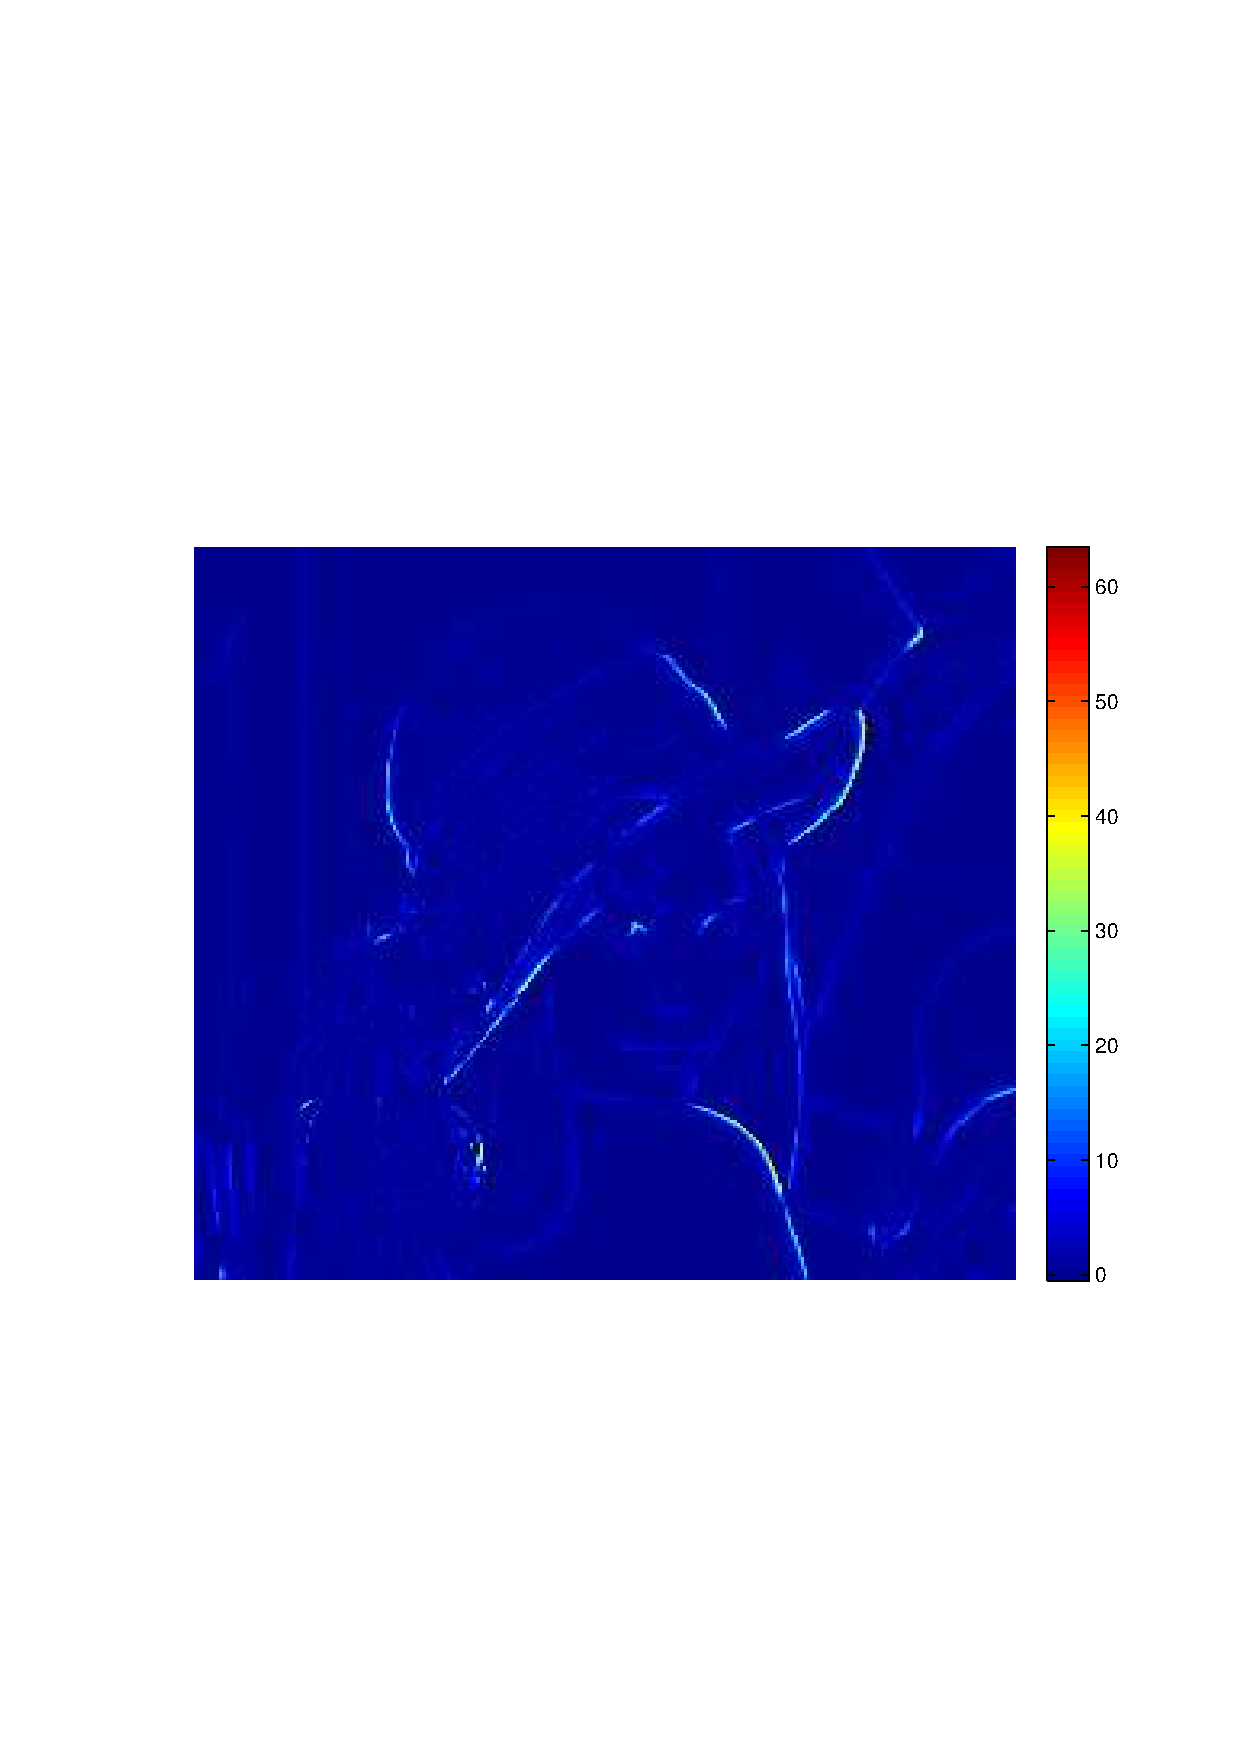
\includegraphics[width=\linewidth]{5zhang2}
    %\captionsetup{skip=1pt}
    \caption{Zhang~\cite{Zhang_2012_TIP}}
    \label{fig:minimax_path:path}
\end{subfigure}
\begin{subfigure}[b]{0.32\linewidth}
    \centering
    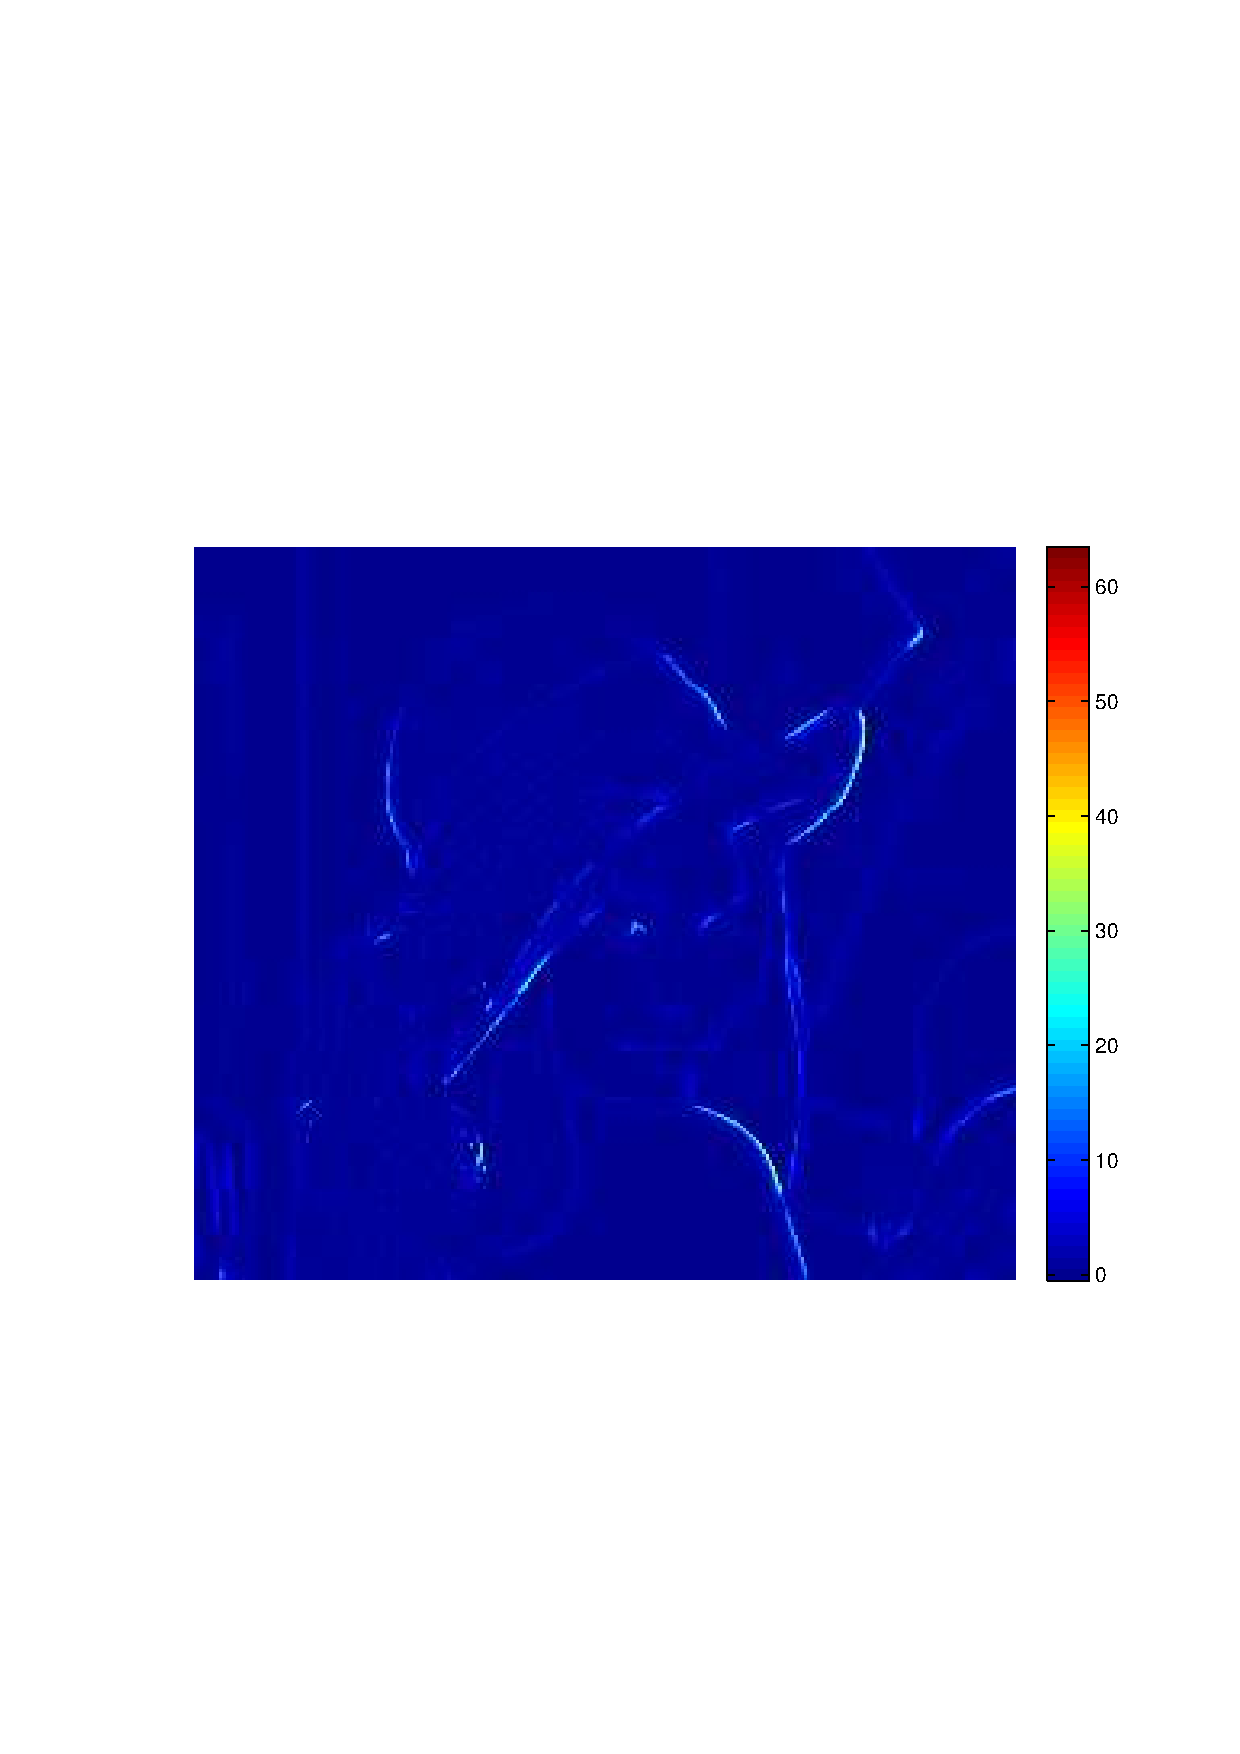
\includegraphics[width=\linewidth]{5Gunturk2}
    %\captionsetup{skip=1pt}
    \caption{Gunturk~\cite{Gunturk_TIP_2011}}
    \label{fig:minimax_path:path}
\end{subfigure}
\begin{subfigure}[b]{0.32\linewidth}
    \centering
    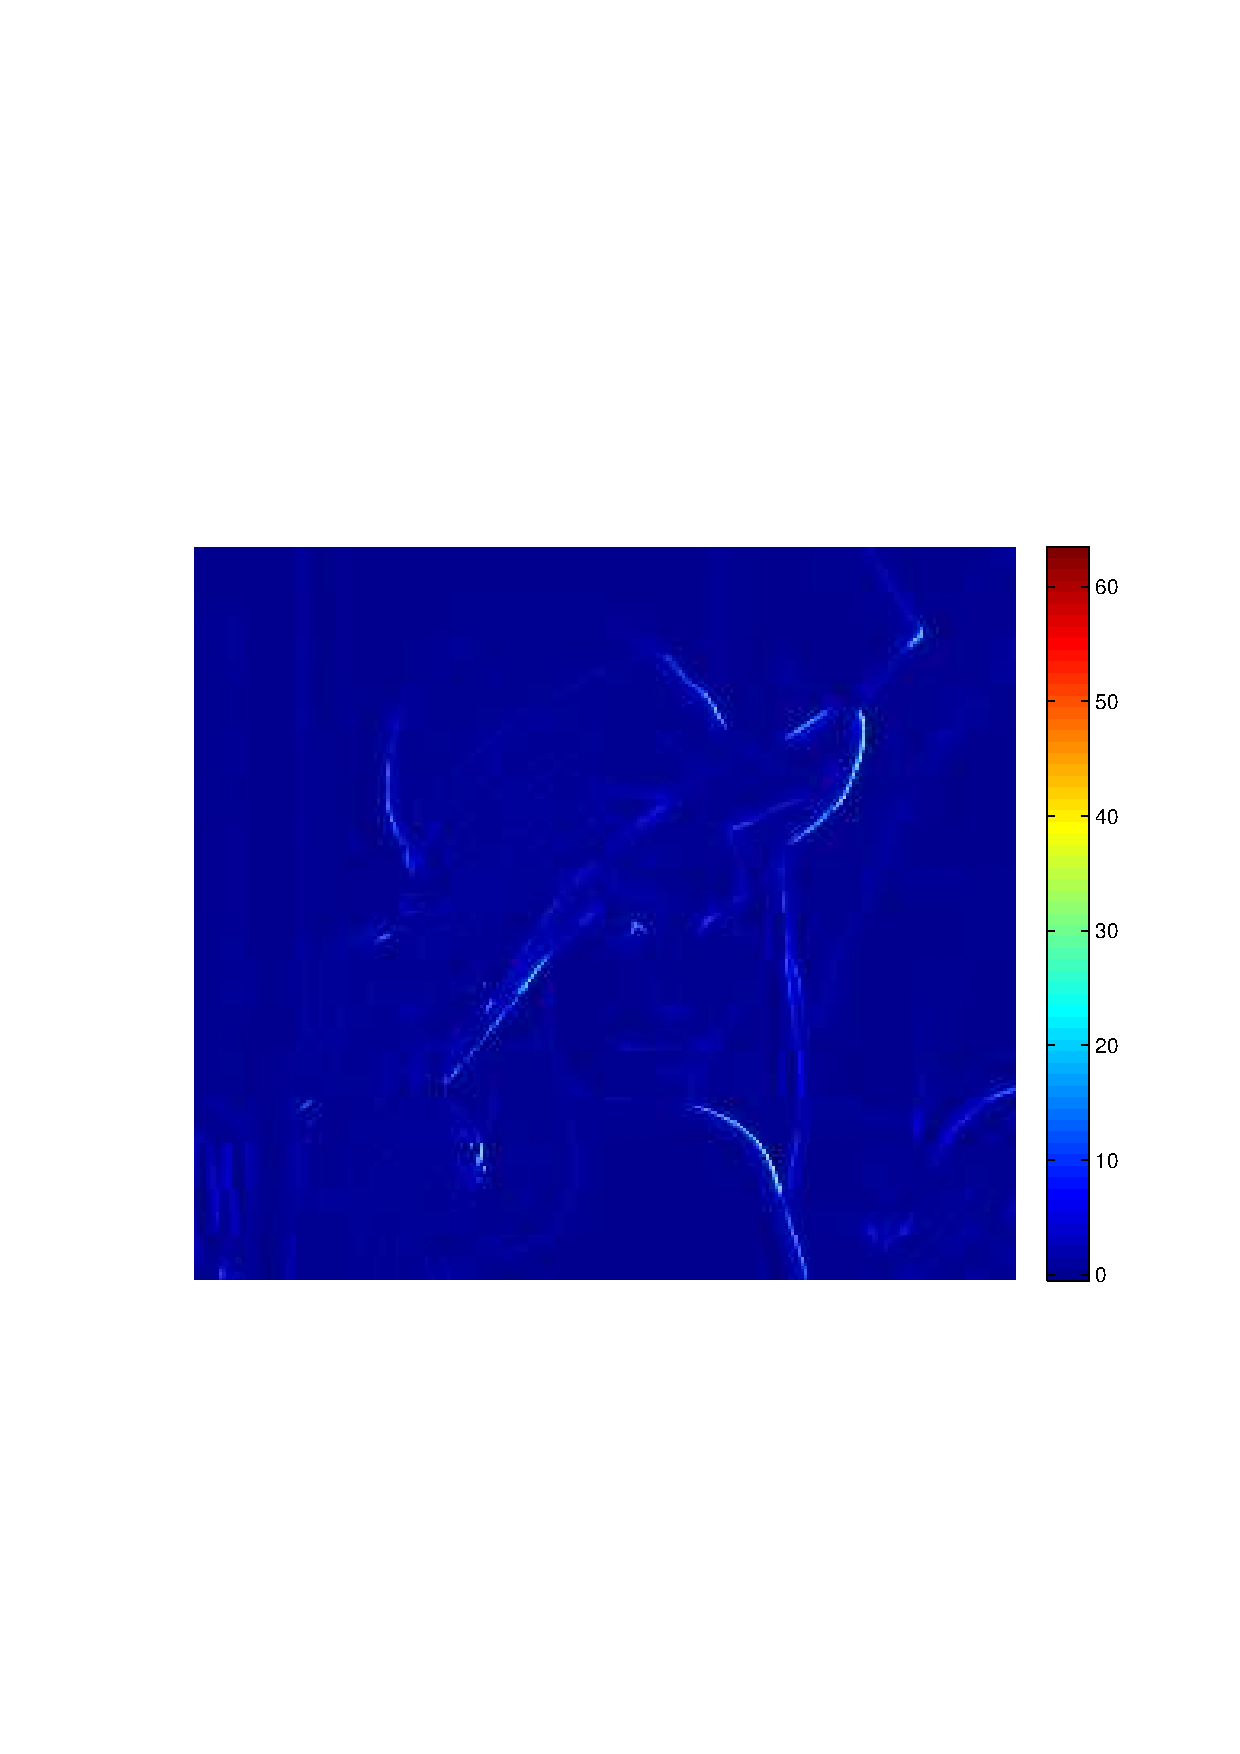
\includegraphics[width=\linewidth]{5Pan2}
    %\captionsetup{skip=1pt}
    \caption{Pan~\cite{Pan_MPE_2014}}
    \label{fig:minimax_path:path}
\end{subfigure}

\begin{subfigure}[b]{0.32\linewidth}
    \centering
    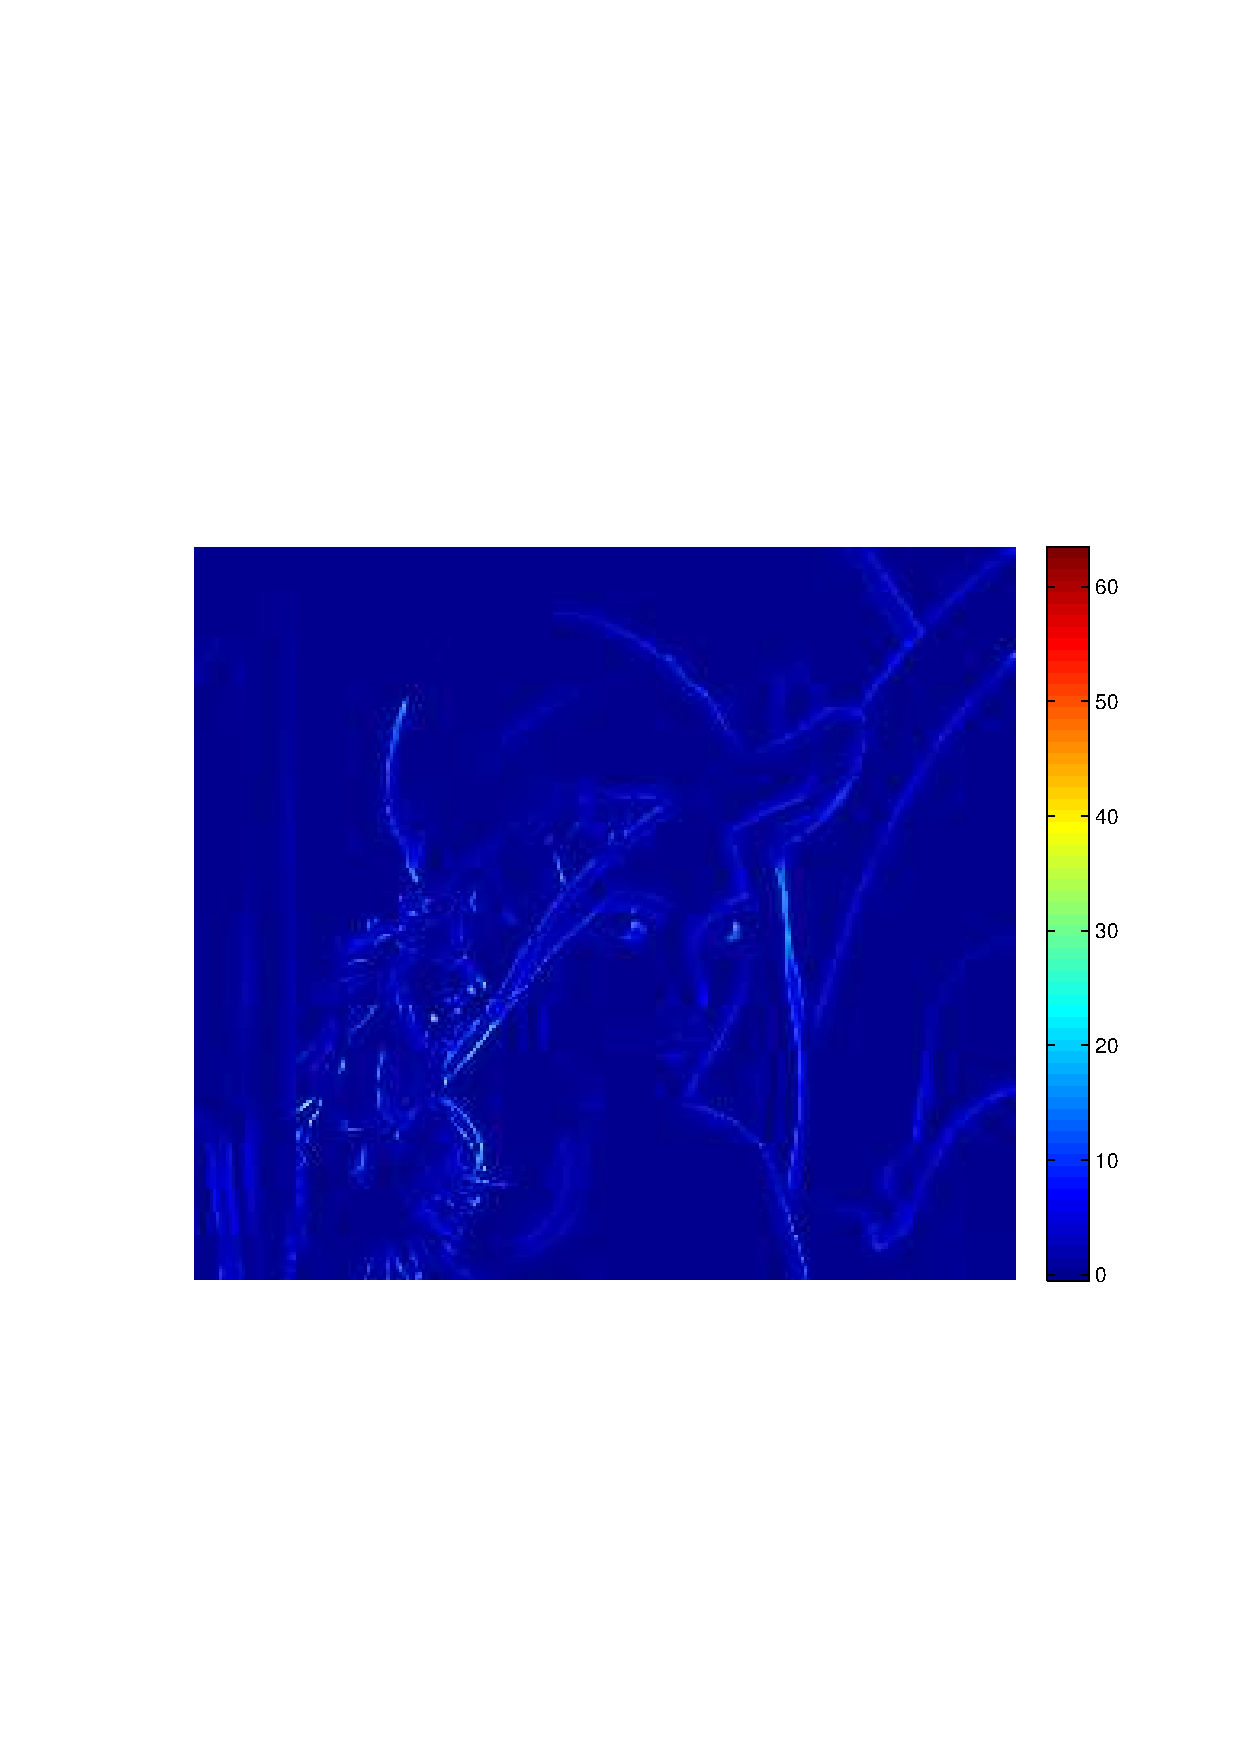
\includegraphics[width=\linewidth]{5Porikli2}
    %\captionsetup{skip=1pt}
    \caption{Dai~\cite{Dai_ET_2014}}
    \label{fig:minimax_path:path}
\end{subfigure}
\begin{subfigure}[b]{0.32\linewidth}
    \centering
    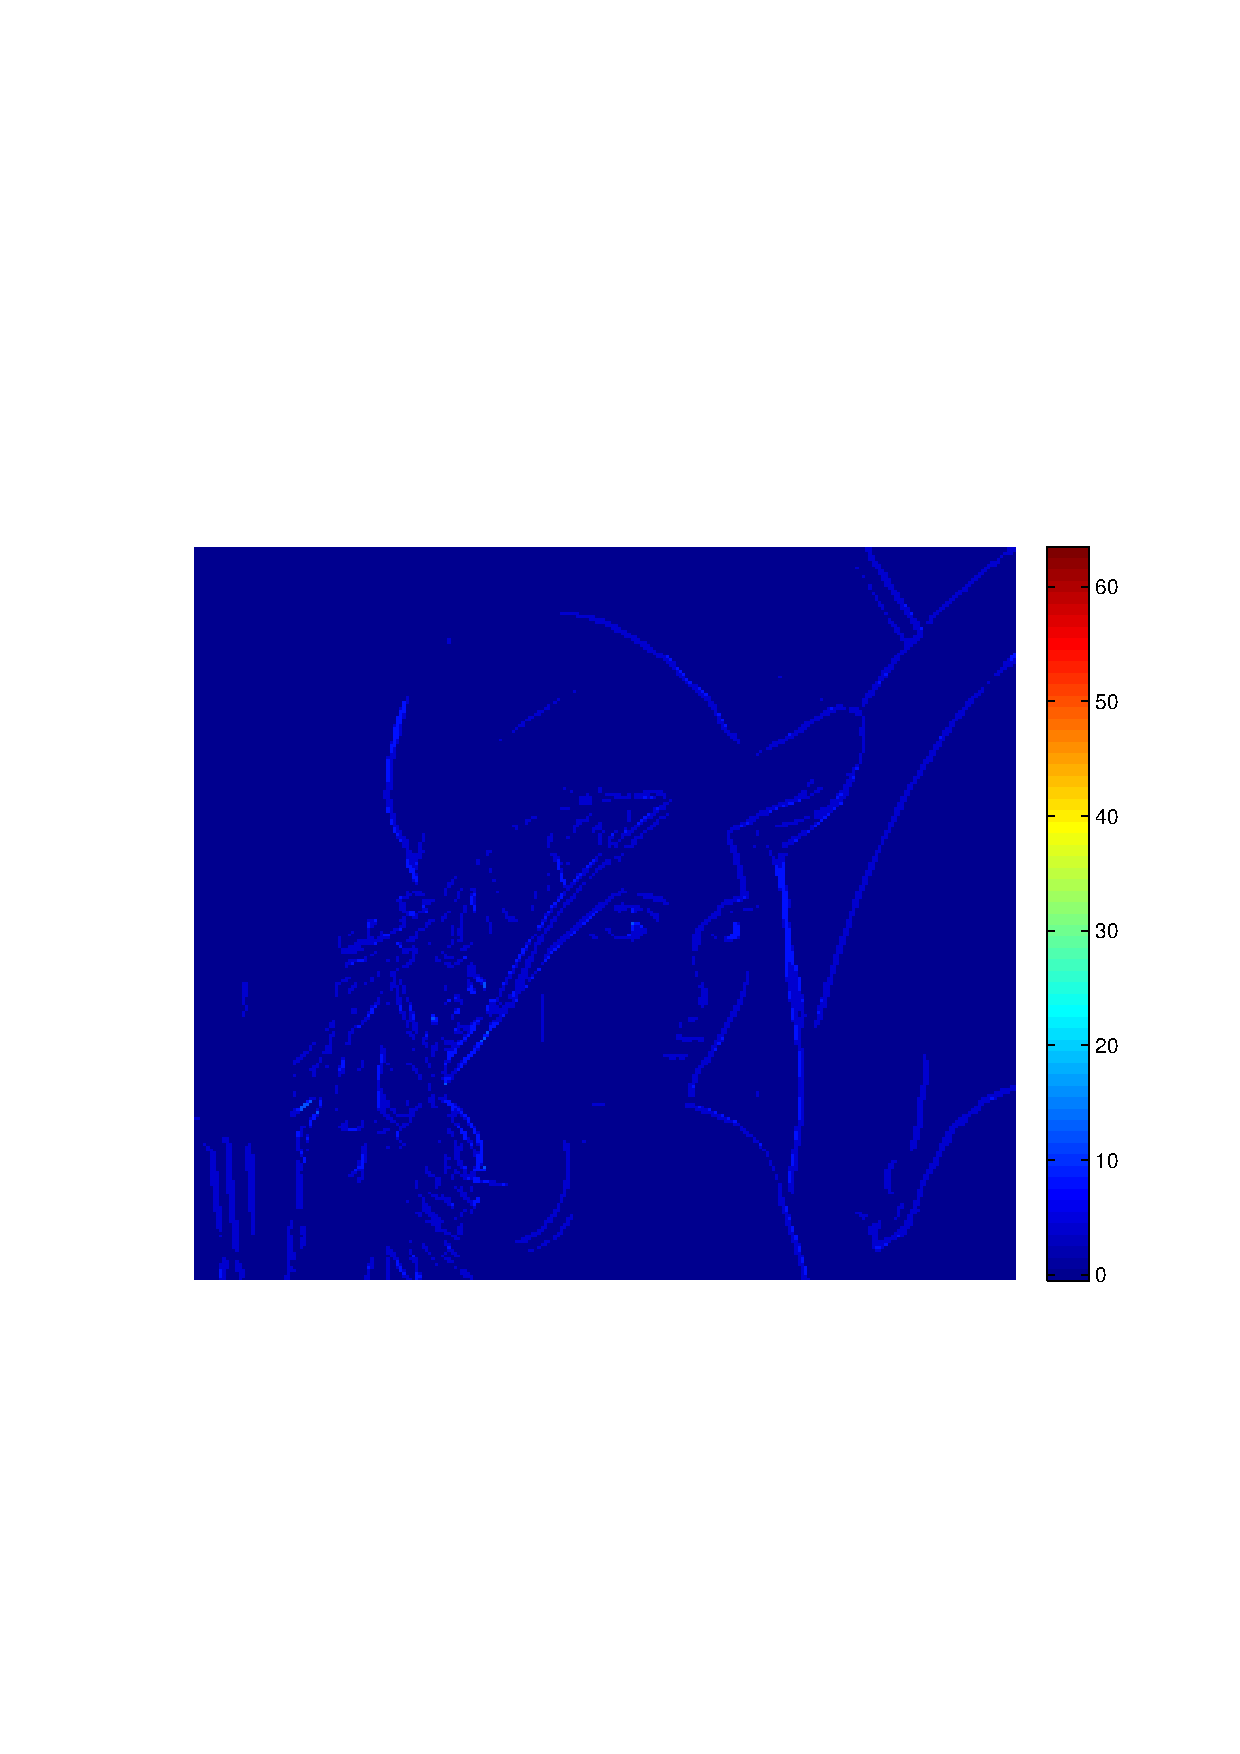
\includegraphics[width=\linewidth]{5Chaudhury2}
    %\captionsetup{skip=1pt}
    \caption{Chaudhury~\cite{Chaudhury_TIP_2011}}
    \label{fig:minimax_path:path}
\end{subfigure}
\begin{subfigure}[b]{0.32\linewidth}
    \centering
    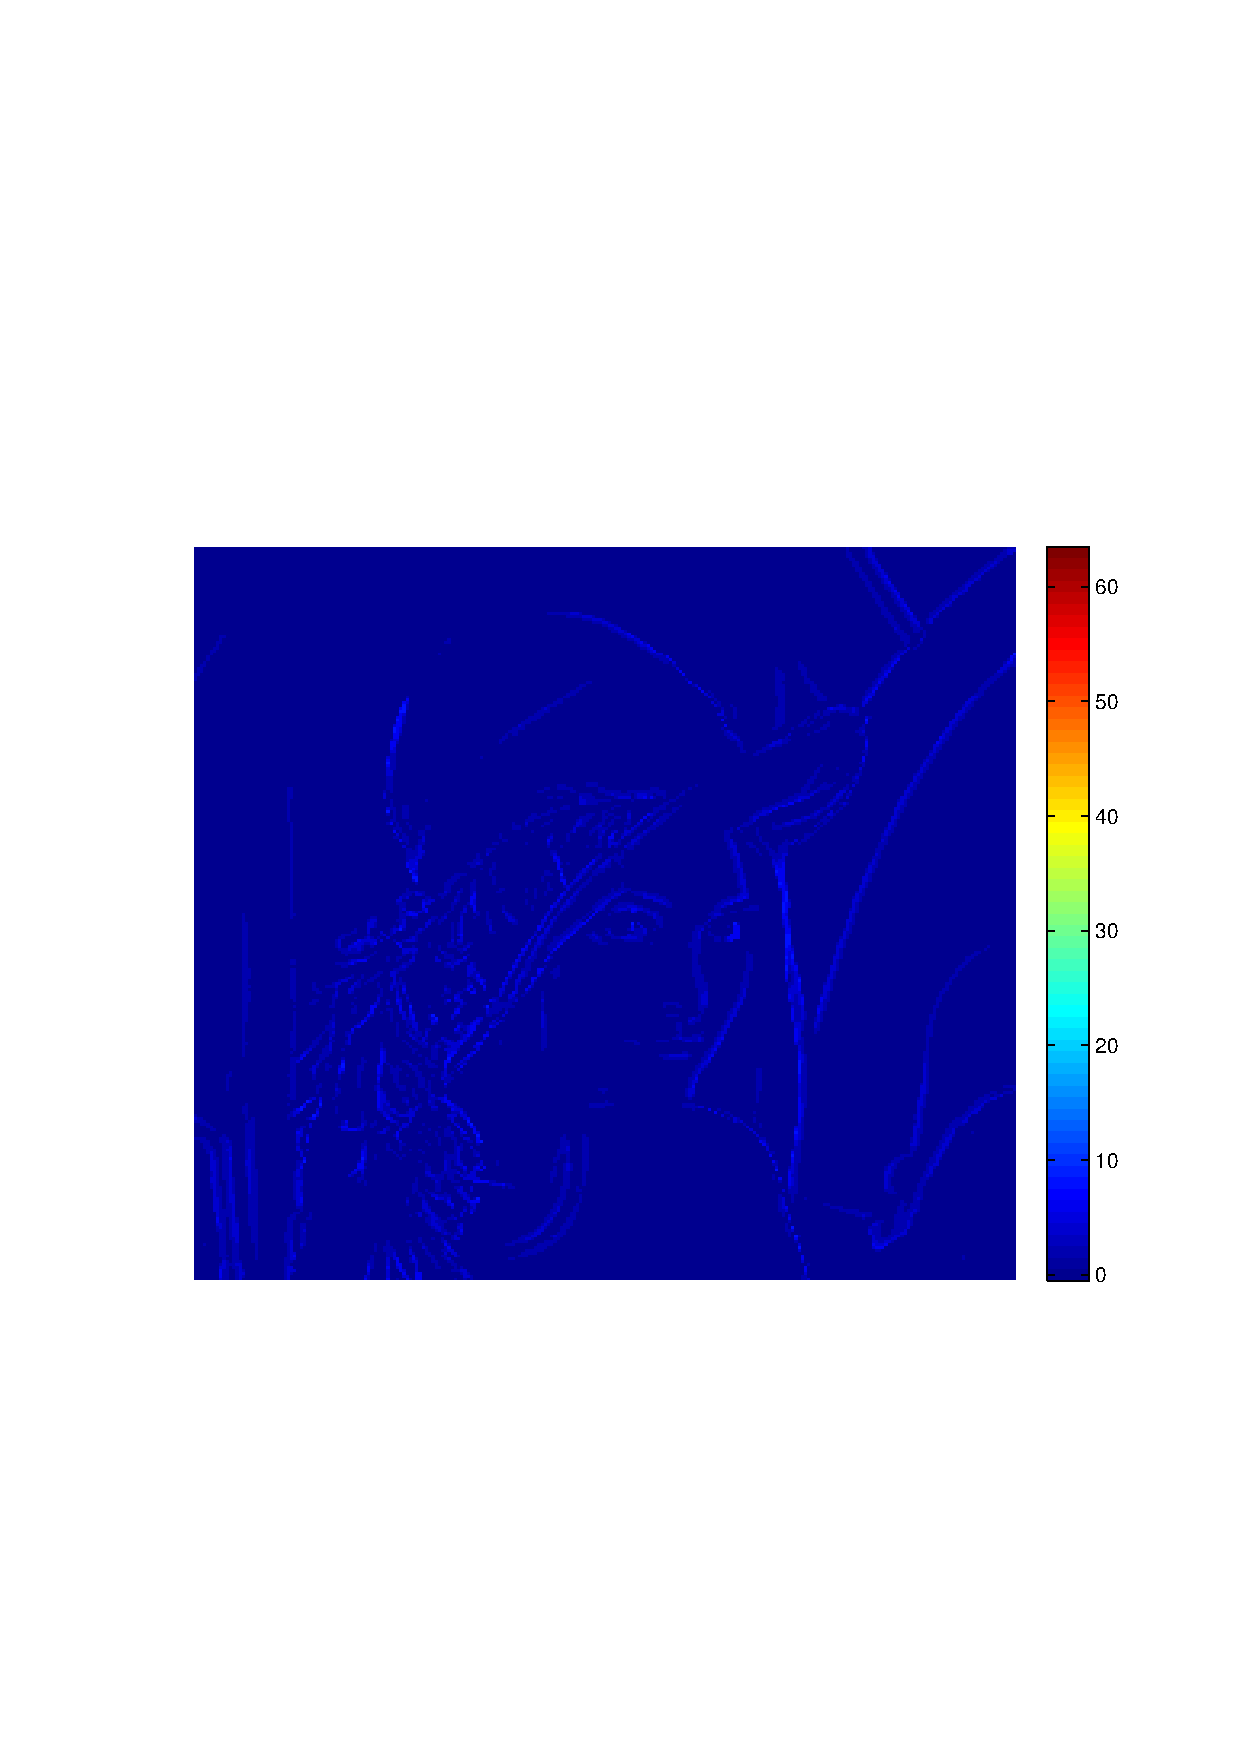
\includegraphics[width=\linewidth]{5Ours2}
    %\captionsetup{skip=1pt}
    \caption{Ours}
    \label{fig:minimax_path:path}
\end{subfigure}
\caption{Approximation error illustration.  The spatial kernel and the range kernel of the prototype BF are chosen as the Gaussian kernel and we assign $\sigma_r = 80$ for the Gaussian range kernel.  }
\label{fig:approximation_error}
\vspace{-0.1cm}
\end{figure}

In this section, we directly compute the linear convolution of $K_s$ and evaluate the PSNR index which reflects the accuracy of different nonlinear convolution decomposition methods to verify the approximation ability of our method. This is because BF accelerating methods adopt various techniques to decompose the nonlinear convolution of the range kernel into a set of the linear convolutions and employ linear time algorithms to fast compute the linear convolutions. If we take the brute-force method to compute linear convolution, the approximation error can only be caused by the nonlinear convolution decomposition method. In order to provide an intuitive illustration, we visualize the approximation error of Lena image in Fig~\ref{fig:approximation_error}. Both the spatial kernel and the range kernel of the prototype BF are chosen to be the Gaussian kernel $G_{\sigma}(\cdot)$. The results are obtained by the naive implementation of the accelerating methods Zhang~\cite{Zhang_2012_TIP},  Gunturk~\cite{Gunturk_TIP_2011}, Pan~\cite{Pan_MPE_2014},  Dai~\cite{Dai_ET_2014},  Chaudhury~\cite{Chaudhury_TIP_2011} and ours without using the brute-force linear convolution. Let $I^{bf}$ denote the result of the naive implementation of BF and $I^{ac}$ represent the result of accelerating methods, we compute the absolute error by $|I^{bf} - I^{ac}|$ and illustrate the filtering results and corresponding absolute error in Fig~\ref{fig:approximation_error}. It is easy to find that our method achieves the smallest absolute error among the six comparative accelerating methods.
%The results of the histogram based BF are very similar because they use the same nonlinear convolution decomposition methods.


\section{Conclusion}

The key of accelerating BF is to decompose the nonlinear convolution of BF into a set of linear convolutions. We do this by substituting the range kernel with the optimal fitting polynomial and then employing the shiftable property to decompose the nonlinear convolution into a set of linear convolutions. The major advantages of our method are that it is able to approach both differential and nondifferential range kernels and our accelerating algorithm only needs addition and multiplication operations to calculate filtering results.
%\vskip3pt
%\ack{This work was supported by the National Natural Science Foundation of China (No. 61332017, 61331018, 91338202, and 61271430).}
\vskip3pt
\noindent Longquan Dai, Mengke Yuan and Xiaopeng Zhang (\textit{NLPR, Institute of Automation Chinese Academy of Sciences, Beijing, China})
\vskip3pt

\noindent E-mail: xiaopeng.zhang@ia.ac.cn


\begin{thebibliography}{}
\bibitem{Tomasi_ICCV_1998}
C.~Tomasi and R.~Manduchi. Bilateral filtering for gray and color images. In \emph{ICCV}, 1998.
	
\bibitem{Chaudhury_SPL_2011}
K.N. Chaudhury, Constant-Time Filtering Using Shiftable Kernels. \emph{IEEE Signal Processing Letters}, 2011

\bibitem{Dai_ET_2014}
Longquan  Dai, Mengke Yuan and Xiaopeng Zhang, Accelerate bilateral filter using Hermite polynomials. \emph{Electronics Letters}, 2014.


\bibitem{Chaudhury_TIP_2011}
K.N. Chaudhury, D.~Sage, and M.~Unser. Fast o(1) bilateral filtering using trigonometric range kernels. \emph{TIP},  2011.

\bibitem{Porikli_2008_CVPR}
F.~Porikli. Constant time o(1) bilateral filtering. In {\em CVPR},
  pages 1--8, June 2008.

\bibitem{Porikli_CVPR_2005}
F.~Porikli. Integral histogram: a fast way to extract histograms in cartesian
  spaces. In {\em CVPR},
  volume~1, pages 829--836 vol. 1, June 2005.

\bibitem{Zhang_2012_TIP}
K.~Zhang, G.~Lafruit, R.~Lauwereins, and L.~Van~Gool.
 Constant time joint bilateral filtering using joint integral
  histograms.
 {\em TIP}, 21(9):4309--4314, Sept
  2012.

\bibitem{Gunturk_TIP_2011}
B.~Gunturk.
Fast bilateral filter with arbitrary range and domain kernels.
 {\em TIP}, 20(9):2690--2696, Sept
  2011.

\bibitem{Pan_MPE_2014}
X.~A. Shengdong~Pan and H.~He.
 Optimal o(1) bilateral filter with arbitrary spatial and range
  kernels using sparse approximation.
 {\em MPE}, 2014.

\bibitem{Durand_2002_TOG}
F.~Durand and J.~Dorsey.
Fast bilateral filtering for the display of high-dynamic-range
  images.
{\em TOG}, 21(3):257--266, July 2002.

\end{thebibliography}

\end{document} 